\documentclass[
	%parspace, % Térköz bekezdések közé / Add vertical space between paragraphs
	%noindent, % Bekezdésének első sora ne legyen behúzva / No indentation of first lines in each paragraph
	%nohyp, % Szavak sorvégi elválasztásának tiltása / No hyphenation of words
	%twoside, % Kétoldalas nyomtatás / Double sided format
	%draft, % Gyorsabb fordítás ábrák rajzolása nélkül / Quicker draft compilation without rendering images
	%final, % Teendők elrejtése / Set final to hide todos
]{elteikthesis}[2021/09/20]

\usepackage{eso-pic}
\usepackage{hyperref}
\usepackage{array,multirow}
\usepackage{longtable}
\usepackage{wrapfig}
\usepackage{hyperref}
%FIGURES AND TABLES
\usepackage{caption}
\usepackage{graphicx}						
\usepackage[section]{placeins}								
\usepackage{booktabs}
\usepackage{float}
\usepackage{lipsum}  
\renewcommand{\thechapter}{\Roman{chapter}}
\renewcommand{\chaptername}{tétel}
\renewcommand{\thesection}{\Alph{section}} 

\newcommand\BackgroundPic{%
	\put(0,0){%
		\parbox[b][\paperheight]{\paperwidth}{%
			\vfill
			\centering
			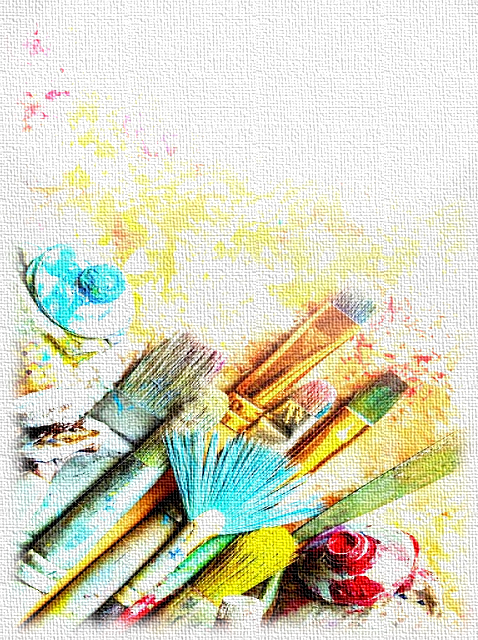
\includegraphics[width=\paperwidth,%
			keepaspectratio]{images/cover.png}%
			\vfill
}}}
% A dolgozat
% The document
\begin{document}

\AddToShipoutPicture*{\BackgroundPic}
\begin{titlepage}
	\AddToShipoutPicture*{\BackgroundPic}		
	\centering
	\begin{figure}[!h]
		\begin{minipage}{0.2\textwidth}
			\centering
			
\includegraphics[width=1.0\linewidth]{images/jaschik_logo}
			\captionsetup{labelformat=empty}	
			\caption{\centering}
		\end{minipage}\hfill
		\begin{minipage}{0.75\textwidth}
			\centering			
			{\scshape\LARGE\bfseries Jaschik Álmos Művészeti Szakgimnázium és Technikum\par}
			\vspace{0.5cm}
			{\scshape\bfseries\Large Képző- és iparművészeti munkatárs\\
				- Festő\par}
		\end{minipage}	
		\captionsetup{labelformat=empty}
	\end{figure}
	\vspace{2.5cm}	
	{\LARGE\bfseries Kidolgozott vizsgatételek\par}
	\vspace{0.5cm}
	{\Large Készítette:\par}
	{\Large\itshape Csonka Szilvia\par}
	{\large\itshape 2022, Budapest\par}
	
\end{titlepage}

% Nyelv kiválasztása
% Set document language
\documentlang{magyar}
%\documentlang{english}

% Teendők listája (final dokumentumban nincs)
% List of todos (not in the final document)
%\listoftodos[\todolabel]

% Tartalomjegyzék (kötelező)
% Table of contents (mandatory)
\tableofcontents
\cleardoublepage

% Tartalom
% Main content
\chapter{Bevezetés: Tételek} % Introduction
\label{ch:bevezetes}

\cleardoublepage

\chapter{Az ókori Egyiptom művészete} % Introduction
\label{ch:1_okri_egyiptom}

\section{Az ókori egyiptom társadalmi felépítése, hiedelemvilága, művészeti korszakai és emlékei}

\vspace{0.5cm}

\tcbox[left=0mm,right=0mm,top=0mm,bottom=0mm,boxsep=0mm,
toptitle=0.5mm,bottomtitle=0.5mm,title=\centering{A tétel adatai}]{%
	
	\begin{tabular}{| p{0.25\textwidth} | p{0.75\textwidth} |}
		
		\centering{\textbf{Tétel teljes címe}}
		&
		Mutassa be az ókori Egyiptom társadalmi felépítését, hiedelemvilágát! Ismertese az ókori egyiptomi művészet korszakait, az építészet, szobrászat és festészet ránk maradt emlékeinek jellegzetességeit!
		\\\hline
		
		\centering{\textbf{Jegyzetek}}
		&
		\begin{compactitem}
			\item Az ókori egyiptomi művészet korszakai, földrajzi, társadalmi környezete.
			\item A sír- és templomépítészet típusai, felépítése, jellemzői.
			\item A szobrászat, a festészet és tárgykultúra jellemzői és stílusjegyei.
		\end{compactitem}
\end{tabular}}\hfill

\subsection*{Földrajzi elhelyezkedés}

\begin{figure}[H]
	\centering
	\tcbox[colback=gray!85!black,
	left=0mm,right=0mm,top=0mm,bottom=0mm,boxsep=1mm,toptitle=0.5mm,bottomtitle=0.5mm,
	title=\centering{Az ókori Egyiptom a Nílus mentén feküdt}]{
		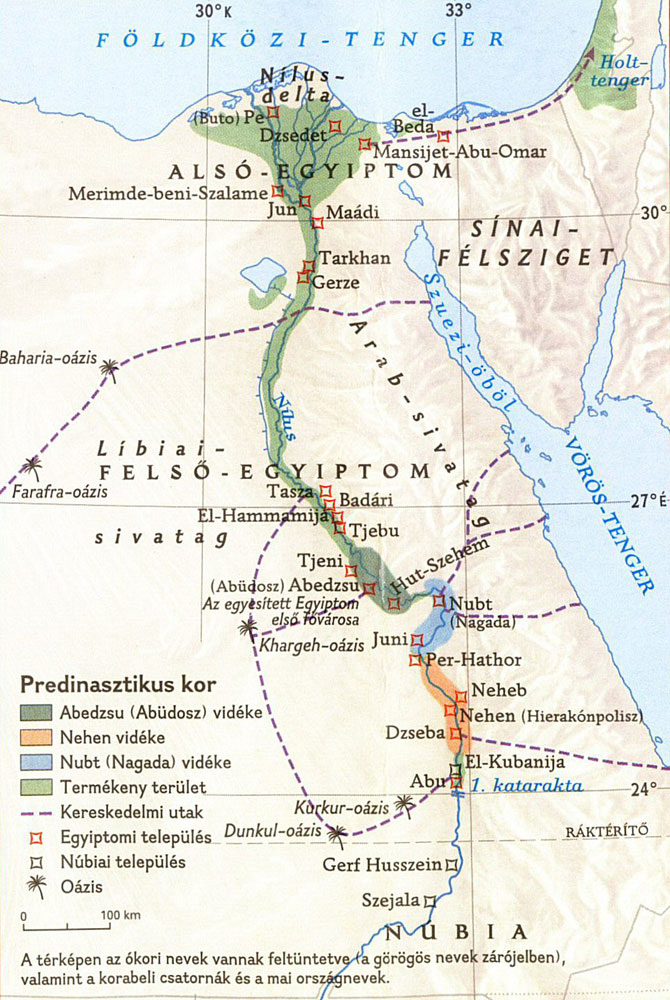
\includegraphics[width=0.9\linewidth]{images/01/egyiptom_terkep}}
	\captionsetup{labelformat=empty}
	\caption{}
\end{figure}

Egyiptom éghaljata alapvetően sivatagos, ezért a kultúra a \textbf{Nílus mentén}, annak partján 5-10 km-es szélességben, több mint 1 000 km hosszan alakult ki.

Ezen ókori civilizáció kialakulásának feltétele a folyó éltető ereje volt: a Nílus. A folyó vetés előtt, júliustól novemberig áradt, termékeny iszapot terítve szét, tápanyagban gazdaggá téve a talajt és lehetővé tette az \textbf{elárasztásos gazdálkodás}t.

A terület földrajzilag és kezdetben politikailag is két részre tagolódott. \textbf{Alsó Egyiptom} északon, a Nílus deltatorkolatánál feküdt a sík vidéken. \textbf{Felső Egyiptom} attól délebbre, a magasabban fekvő területeken, a Nílus mentén hosszan kanyargó partszakaszon helyezkedett el.

\subsection*{Társadalmi felépítés}

\begin{tcolorbox}[enhanced,colframe=gray!50!white,
	colbacktitle=gray!15!white,
	coltitle=gray!50!black,
	borderline={0.5mm}{0mm}{gray!15!white},
	borderline={0.5mm}{0mm}{gray!50!white,dashed},
	attach boxed title to top center={yshift=-2mm},
	boxed title style={boxrule=0.4pt},
	title=Az ókori Egyiptom társadalmi felépítése]{
			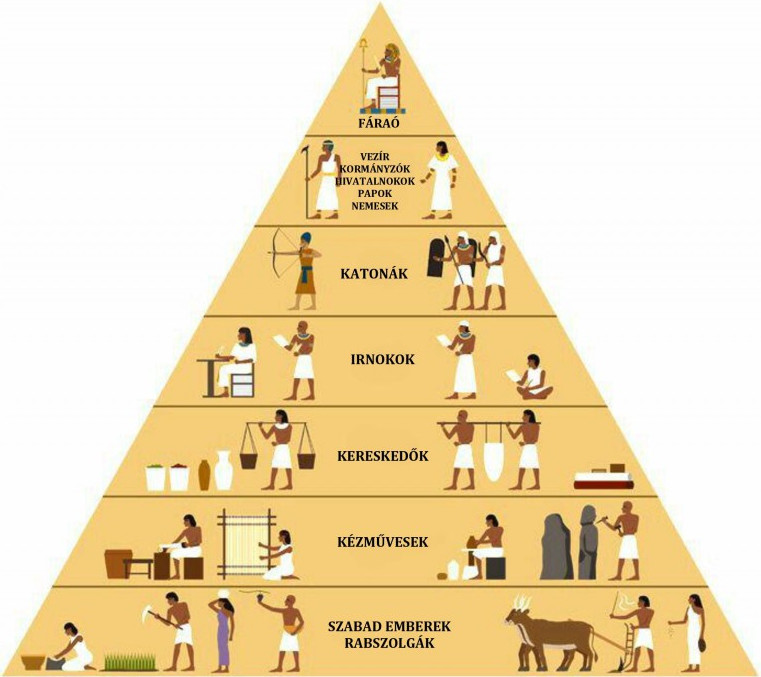
\includegraphics[width=1.0\linewidth]{images/01/egyiptomi_tarsadalom}}
\end{tcolorbox}

Az állam élén a korlátlan hatalommal rendelkező \textbf{fáraó} állt. Az előkelőket a származás szerinti arisztokrácia alkotta, belőlük kerültek ki a főtisztviselők. Az államigazgatás és az igazságszolgáltatás vezetője a vezér. A gazdasági élet irányítószerve a kincstár, az államgépezet működését az írnokok biztosították.

A közigazgatási egységek a nomoszok (kerületek), élükön a nomarkhoszokkal (kormányzókkal). A közrendűeket két réteg alkotta: a parasztok - a föld használata fejében terménnyel és közmunkával adóztak -, és a kézművesek. A házi rabszolgák a hadifoglyokból kerültek ki.\\

\begin{compactitem}
	
	\item\textbf{ Fáraó}: a trón betöltése általában a primogenitura elve (elsőszülött öröklése) történik.\\
	\textit{A fáraó volt a hadsereg főparancsnoka, az államigazgatás és a kincstár feje, valamenynyi templom főpapja és a legfőbb bíró. Mindezeken túl úgy gondolták, hogy rajta múlik az ország termékenysége. Ő tette a földeken az első kapavágást, és ő kezdte meg az aratást.}
	
	\item\textbf{ Papi arisztokrácia}\\
	\textit{A papok - egyiptomi felfogás szerint - csupán az uralkodót helyettesítették kultikus funkcióiban. Hisz a legfőbb pap a fáraó volt! Az egyiptomi papság két fontos funkciót látott el: az istenek kultuszának szolgálatát a templomokban és a halottakról való gondoskodást, az áldozatok bemutatását.}
	
	\item \textbf{Katonai arisztokrácia}\\
	\textit{A fáraó hatalmának alapja a felügyelete alatt álló oikosz-gazdaság és a zsoldos hadsereg volt mely akatonai arisztokrácia megszilárdulásával vált lehetővé. A katonai tisztségviselők elsősorban a társadalom tehetősebb képviselői voltak: előkelők, nagyobb földbirtokosok.}
	
	\item \textbf{ Írnokok} (tisztviselők) (nyilvántartás, adóztatás)\\
	\textit{Az egyiptomi állam legfontosabb hivatalnoka volt. Az irnokok készítették a legfontosabb feljegyzéseket, összeírásokat, a különböző vallási, orvosi, irodalmi szövegeket. Az írástudás minden hivatal elnyerésének feltétele volt. Egy-egy előkelő tucatnyi irnokot foglalkoztatott, s az írnokból akár magas méltóság is válhatott.}
	
	\item \textbf{Kézművesek}\\
	\textit{A Der-el-Medinában élő, kézműves férfiaknak és nőknek tíz napos időszakokra el kellett hagyniuk a várost és családjukat, hogy dolgozni menjenek oda, ahová a fáraó és legfőbb tanácsadói parancsolták. Rövid pihenési időszak után a munkások újabb tíz napot dolgoztak.}
	
	\item\textbf{ Közrendű szabadok}\\
	\textit{A közrendű szabadok foglalkozás szerint földművesek, kézművesek és kereskedők lehettek. A "félszabadok" az ún. királyi munkások, a földbirtokhoz kötött - főleg - parasztok.
	Fontos tény továbbá, hogy a piramisokat nem rabszolgák építették, hanem a közrendű, szabad népesség.}

	\item \textbf{Parasztok}: középítkezések az áradások idején
	
	\item \textbf{Rabszolgák}\\
	\textit{A rabszolgák döntően hadjáratok folyamán kerültek Egyiptomba. Már az i.e. 2700 kö-rül keletkezett „ palermói kő „ is beszámolt arról, hogy egy núbiai hadjárat  után 7000 foglyot hurcoltak az országba.}
\end{compactitem}

\vspace{0.5cm}

Az ókori egyiptomiak úgy hitték, hogy hajdanában nem voltak földi királyok, hanem maguk az istenek uralkodtak az ország felett. Ozirisz volt az, aki földművelésre tanította az embereket. Az ő felesége volt Ízisz, fiuk pedig Hórusz, a sólyomisten. A hór szó valójában magasröptűt, magasságot is jelentett, ezért származtatták magukat tőle az uralkodók. \textbf{Az egyiptomiak királyaikat tehát az istenek földi képviselőjének tekintették.}

\subsection*{Írásmód}

	\begin{wrapfigure}{r}{0.23\textwidth}
		\tcbox[colback=darkgray!85!black,
		left=0mm,right=0mm,top=0mm,bottom=0mm,boxsep=1mm,toptitle=0.5mm,bottomtitle=0.5mm,
		title=\centering{A rosettei kő}]{
		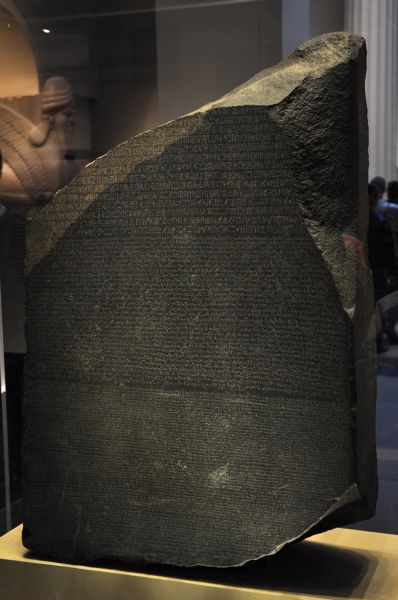
\includegraphics[width=1.0\linewidth]{01/rosetti_ko}
	}
	\end{wrapfigure}

	A legismertebb írásmód a \textbf{hieroglifa} (a szó görög eredetű és „szent vésetet” jelent), \textbf{elsősorban a falakra került és a kultuszhoz} [= a vallásgyakorlat, a vallásos szertartások összessége] \textbf{kapcsolódott}.
	
	Maguk az egyiptomiak írásukat a \textit{medu netjeru}, „az istenek szavai” névvel illették, ezzel is utalva a legendára, mely feltalálását Thot istennek tulajdonítja.
	A hieroglifa-írást 1822-ben fejtette meg Francois Champollion [sampolion] francia tudós, az ún. rosette-i kő alapján, amely egy olyan kőtábla volt, amin ugyanaz a szöveg három nyelven volt olvasható többek közt görög betűkkel.
	
	\begin{tcolorbox}[enhanced,colframe=gray!50!white,
		colbacktitle=gray!15!white,
		coltitle=gray!50!black,
		borderline={0.5mm}{0mm}{gray!15!white},
		borderline={0.5mm}{0mm}{gray!50!white,dashed},
		attach boxed title to top center={yshift=-2mm},
		boxed title style={boxrule=0.4pt},
		title=A hieroglif írás]{
			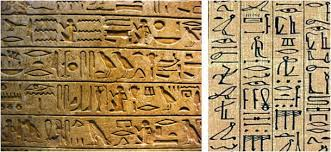
\includegraphics[width=1.0\linewidth]{images/01/hieroglifa}}
	\end{tcolorbox}

	Az írás leggyakoribb alapanyaga - a sírfalakon kívül - a papirusztekercs volt. A háromszög keresztmetszetű papirusznád belső rostjait kivették, hosszú csíkokra vágták, 6 napig vízbe áztatták, függőlegesen majd ezekre keresztbe egymásra helyezték a csíkokat (tulajdonképpen egy fonatot hoztak létre). Majd újabb 6 napon keresztül összepréselték, kiszárították, végül a lapokat a végüknél egymáshoz ragasztották, így jött létre az összegöngyölhető tekercsforma a könnyebb tárolhatóság érdekében.
	

\subsection*{Hiedelemvilág}

Az egyiptomiak egyes természeti jelenségekben természetfölötti erőknek a megtestesülését látták, melyet a hieroglif írásban, a művészi ábrázolásokban emberi, állati, növényi vagy akár egy tárgy alakjában mintáztak meg. 

Egy-egy isten megjelenhetett nemcsak emberi, hanem állati alakban is, sőt nagyon gyakran az emberi testet állatfejjel olvasztották egybe. Ugyancsak lényeges volt az istenek elnevezése is, ami jellemezte viselőjét: az Elrejtett, az Alkotó, a Hatalmas, stb. A vallásos hiedelmek között nagy szerepe volt a mágiának, hisz az egyiptomiak felfogása szerint egy természetfeletti erő igénybe vétele kellett mindenféle baj, veszedelem, betegség leküzdéséhez. Ilyen természetfeletti erőt tulajdonítottak a különböző varázsszövegeknek.

Elképzelésük szerint a fáraó, akit Hórusz földi helytartójának tartottak szintén varázserőt sugárzott. A fáraónak a napisten, Ré fiaként való tisztelete az Óbirodalom közepétől vált általánossá.

Az isteni erők sokféleképpen való megtestesítése mellett az egyiptomi vallás egyik legjellemzőbb részei a \textbf{napkultusz} és a \textbf{halottkultusz}. Ahogy a földi élet \textbf{Ré} (napisten) napsugarainak eredménye, úgy a halál utáni továbbélés, a fennmaradás lehetőségét az Ozirisz-hit adta, s ennek része volt a mumifikálás, amivel a halott túlvilági életét akarták biztosítani.

Az egyiptomi vallás egészén két tényező hatása vonul át: a szellemhité, mely mint lélekhit az egyiptomiak páratlanul fejlett halott- és őskultuszát táplálja; továbbá a vele párosult varázslaté, mely áthat a vallásra, átalakítja az istenek erejéről való felfogást, az isteneket aláveti a varázsszövegeknek, a halottakat mentesíti az erkölcsi felelősség alól az ítéleten, alapjává lesz a király és az egyedek istenné válásának.

A vallás gyakorlásának helyei a templomok voltak, melyek egyben iskoláikkal, könyvtáraikkal a tudománynak, a művelődésnek és a teológiai irodalomnak is a centrumaiként szolgáltak.

\subsubsection*{Többistenhit, fontosabb istenek}

\begin{compactitem}
	\item \textbf{Ré} (vagy Rá, kérdéses): napisten, az emberiség atyja.
	\item \textbf{Hórusz}: az istenek királya a Földön. A mitológiában Ozirisz és Ízisz fia, és az ég ura.
	\item \textbf{Ízisz}: anyaistennő, az Ókori Egyiptom egyik leghíresebb istennője, a varázslás, a termékenység, a víz és szél, a tengerhajózás istennője, a nőiesség és a hűség szimbóluma, Ozirisz felesége, Hórusz anyja.
	\item \textbf{Ozirisz}: a túlvilág birodalmának királya és bírája. Az egyik főisten. Ízisszel és Hórusszal alkot istenháromságot. A túlvilág és a halottak istene, az alvilág életet adó ura, a termőföld istene, ő tanította meg az embert a földművelésre.
	\item Anubisz: az alvilág és holtak oltalmazója, és a bebalzsamozás istene. Fekvő sakál- vagy vadkutyaként ábrázolták, illetve sakál- vagy kutyafejű emberként. Anubisz bíraként van jelen a szív megmérésénél, amikor is a halott szívét egy mérlegre teszik, a másik serpenyőbe pedig Maat-nak, az igazság istenének tollát rakják. Ha a szív nehezebb, akkor azt felfalja Ammut, egy alvilági szörny. Ő tartja számon a holtak szívét.
	\item Széth: a vihar és káosz istene.
	\item Thot (vagy Dzsehuti): a bölcsesség és a Hold istene. Íbiszként vagy kutyafejű páviánként ábrázolták. A civilizációt hozta el az embereknek.
	\item Szobek: az istenek őrzője, krokodilisten.
	\item Hathor, az Égi Tehén: Azonosult Básztettel, a termékenység és a szerelem istennője, tehén képében jelenik meg, Íziszhez hasonlították, bár a két istennő egymástől teljesen különbözött.
	\item Ámon: az istenek királya, ugyanaz mint Ámon-Ré, a napisten.
\end{compactitem}

\vspace{0.5cm}

\begin{tcolorbox}[enhanced,colframe=gray!50!white,
	colbacktitle=gray!15!white,
	coltitle=gray!50!black,
	borderline={0.5mm}{0mm}{gray!15!white},
	borderline={0.5mm}{0mm}{gray!50!white,dashed},
	attach boxed title to top center={yshift=-2mm},
	boxed title style={boxrule=0.4pt},
	title=Az ókori Egyiptom istenei]{
		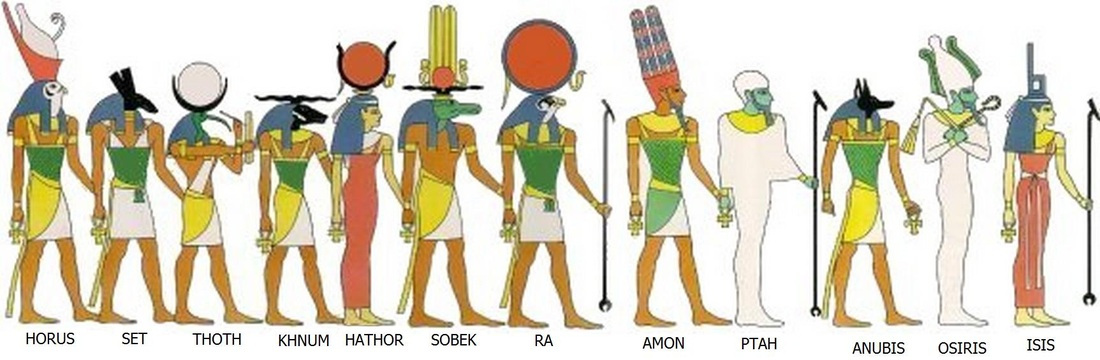
\includegraphics[width=1.0\linewidth]{images/01/istenek}}
\end{tcolorbox}

\subsection*{Halottkultusz, temetkezési szokások}

	Az egyiptomi hitvilág szerint \textbf{az embernek két lelke volt}:\textbf{ az egyik a Ba nevű test-lélek} (tulajdonképpen maga a test), \textbf{a másik a Ka nevű szellemi lélek} (életadó energia, a test állandó tanácsadója, lelkiismerete [ma talán pszichének neveznénk]). A szellemi lélek a vélekedés szerint azonban csak addig él, amíg a testlélek is, ezért a testet meg kellett őrizni az örökkévalóságig, a szellemi lelket pedig táplálni kellett. (A test megőrzését szolgálta a mumifikálás és a masszív sírépületek, a piramisok.) A hitvilág szerint a szellemi lélek minden éjszaka lemegy az alvilágba, majd minden reggel a nappal együtt újjáéled. Az élet tehát mindig Kelethez, a napkeltéhez, a halál mindig Nyugathoz, a naplementéhez kapcsolódott, ezért temetkeztek az egyiptomiak minden korszakban a Nílus bal, azaz nyugati partjára.
	
	\textbf{A test megőrzésének módja a mumifikálás volt.} (Az eljárás kiindulása bizonyára az volt, hogy a predinasztikus korban a száraz sivatagi homokba temetkeztek, ami kiszívta a test nedvességét, ezáltal meggátolta a hús bomlását.) A műveletet papok végezték a sírok mellett lévő halotti templomban:
	\begin{compactitem}
		\item Az elhunyt belső szerveit kivették, kiszárították és az ún. kanopusz-edényekbe helyezték.
		\item Az agyat az orron keresztül eltávolították, a testet és a koponyát gyantával, szurokkal töltötték ki.
		\item A testet tartósító sós lébe áztatták, 70 napig a napon szárították, bebalzsamozták, végül vászonszalagokkal légmentesen bepólyálták.
	\end{compactitem}

\begin{figure}[!h]
	\begin{minipage}{0.49\textwidth}
		\centering
		\tcbox[colback=darkgray!85!black,
		left=0mm,right=0mm,top=0mm,bottom=0mm,boxsep=1mm,toptitle=0.5mm,bottomtitle=0.5mm,
		title=\centering{Kanópuszedények}]{
			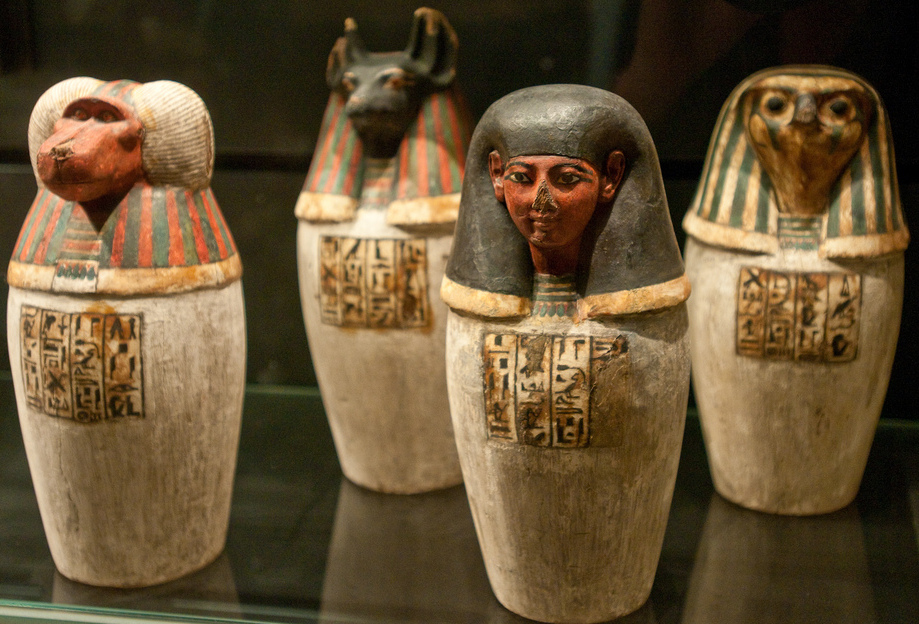
\includegraphics[width=1.0\linewidth]{01/kanopusz}
		}
	\end{minipage}\hfill
	\begin{minipage}{0.45\textwidth}
		\centering
		\tcbox[colback=darkgray!85!black,
		left=0mm,right=0mm,top=0mm,bottom=0mm,boxsep=1mm,toptitle=0.5mm,bottomtitle=0.5mm,
		title=\centering{Múmia ábrázolása}]{
			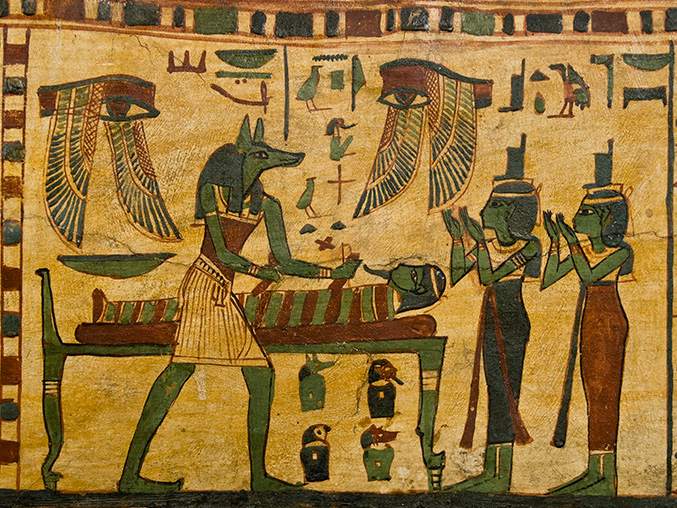
\includegraphics[width=1.0\linewidth]{01/mumia}
		}
	\end{minipage}\hfill
	\captionsetup{labelformat=empty}
	\caption{}
\end{figure}

	

\subsection*{Művészeti és birodalmi korszakok}

	Az egyiptomi művészet nem díszítésre szolgáló vagy történeteket elmesélő művészet volt, hanem kifejezetten gyakorlati funkciót töltött be: a halottkultusz része volt. Az építészetben megjelenő formáknak, a sírfestészet, sírszobrászat témáinak és stílusának mind az egyiptomi hitvilágban, mitológiában találhatjuk meg a magyarázatát.

Egyiptom történelmének nagy részét három „birodalmi” szakaszra lehet osztani (melyek a művészet szempontjából is meghatározóak voltak): az óbirodalmi szakaszra, a középbirodalmi szakaszra és az újbirodalmi szakaszra. Ezeket rövidebb átmeneti időszakok választották el egymástól. Az „átmeneti” szó itt arra utal, hogy ezekben az időkben Egyiptom nem állt egységes politikai uralom alatt, hanem más, erősebb birodalmak uralma alá került. Az egyiptomi civilizáció alapjait jóval az Óbirodalom kora előtt a Nílus folyó partján letelepülő emberek által létrehozott öntözéses földművelés fektette le, amely a városok és specializált gazdasági tevékenységek (például a kézművesség, bányászat) kialakulásához vezetett.\\

\tcbox[left=0mm,right=0mm,top=0mm,bottom=0mm,boxsep=0mm,
toptitle=0.5mm,bottomtitle=0.5mm,title=\centering{Az ókori Egyiptom jelentősebb fáraói}]{
		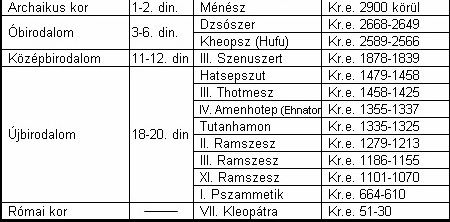
\includegraphics[width=1.0\linewidth]{images/01/faraok}}


\tcbox[left=0mm,right=0mm,top=0mm,bottom=0mm,boxsep=0mm,
toptitle=0.5mm,bottomtitle=0.5mm,title=\centering{Az ókori Egyiptom korszakai}]{%
	
	\begin{tabular}{| p{0.12\textwidth}|p{0.1\textwidth} | p{0.69\textwidth} |}
		
		\centering{\textbf{Óbiro- dalom}}
		&
		kb. Kr. e. 2600-2100
		&
		Híres fáraók: Dzsószer, Kheopsz, Kefrén, Mükerinosz. Kialakul a piramis gúla formája. Gyakran a piramis mellett elhelyezett fáraó szobrok jellegzetes vonásokkal. Hivatalnokok masztabáiból maradtak fenn szobrok és domborművek.
		\\\hline
		
		\centering{\textbf{Közép- birodalom}}
		&
		kb. Kr. e. 2000 - 1700
		&
		Meggyengült a fáraók hatalma, a birodalom kisebb részekre szakadt, délen nomád népek fosztogattak. Théba városa emelkedett ki, ez lett az új, ismét megszilárdult hatalom központja. A sírrablók miatt a piramisok helyett sziklasírokba temetkeztek a fáraók (Királyok völgye).
		\\\hline
		
		\centering{\textbf{Újbiro- dalom}}
		&
		Kr. e. 1600 - 1000
		&
		Rövid, átmenetileg nem egységet időszakot követően Hatsepszut fáraónő kezében központosult a hatalom. A korszak kiemelkedő fáraója IV. Amenhotep, aki Ehnatonra változtatta nevét és bevezette az egyisten hitet: Aton, a Nap mint égistest istenének kultuszát, ez volt az Amarna-kor. Tutanhamon uralkodása alatt visszaállt a régi egyisten hit, egyben ő volt az egyetlen fáraó, akinek szíklasírját érintetlenül találták a régészek. A kor művészeti jellegzetességei a monumentális templomok, amelyek előtérbe kerültek a piramisok helyett: II. Ramszesz Luxori temploma, Karnaki nagy Amon-tempom (több uralkodó is bővítette, III. Amenhotep kezdte el építeni),  a Memnón-kolosszusok melyek a folyóparton épült templomból megmaradtak az áradások után, Hatsepszut fáraónő sziklaegyüttesnek támaszkodó temploma a Királyok völgye mellett.
		\\\hline
		
		\centering{\textbf{Kései kor}}
		&
		K r. e. 722–664
		&
		 Egyiptom hanyatlani kezdett, i.e. IV. században Nagy
		Sándor hódította meg.
		\\\hline
\end{tabular}}\hfill

\clearpage

\subsection*{Az Óbirodalom művészete (kb. Kr.e. 2600-2100)}

Első fáraója Dzsószer volt, majd utána a leghíresebb egyiptomi uralkodók következtek: Kheopsz, majd az ő fia, Kefrén, és unokája Mükerinosz. Az országot ekkor 42 kerületre osztották, melyek élén egy-egy ún. vezír, azaz hivatalnok állt. Ennek az időszaknak a legfontosabb emlékei az említett négy fáraó piramisai Szakkarában és Gízában, a fáraók piramisai és szobrai.

\subsubsection*{Piramis-építészet}

\paragraph{Funkció} A piramisok az egyiptomi uralkodók sír-építményei voltak. Céljuk a halott fáraó mumifikált testének megőrzése volt, valamint hatalmas méreteikkel a fáraó nagyságát szimbolizálták. A piramisok tetején egy aranyból készült piramidion volt: a piramist felül lezáró kissebb piramis (15-20 méter magas). Mivel a nap fényét visszaverte, csillogásával mindenfelé jelezte a hatalmas fáraó sírjának helyét. (Ezek már nincsenek meg.)

\paragraph{Építőanyag} A piramisokat mészkőtömbökből építették, amit helyben bányásztak, és szabályos téglatest formájúra faragtak. A tömbök között semmilyen kötőanyagot nem használtak. A nagyméretű kőtömböket úgy szállították, hogy a sivatagi homokon egy iszap-utat hoztak létre, amin a kőtömb könnyedén csúsztatható volt, mindössze 6 emberre volt szükség így a szállításához. Néhány esetben - a belső kamrákban - gránitot is használtak, ami a legnehezebb és a legkeményebb kőfajta. A kemény kövek használata is kifejezi, hogy a piramisokat az örökkévalóság számára építették.

\paragraph{Építők} A piramisokat építő rabszolgákról Hérodotosz görög történetíró számolt be, ez a nézet azonban mára elavulttá vált: a helyben élő szabad, fölművelő köznép élelem fejében dolgozott a fáraónak azalatt, amíg a Nílus kiáradt. 

A Gízai piramisok mellett megtalálták a munkások városát, ami kórháztól kezdve sörfőzdén át mindennel el volt látva, ami csak a mindennapi élethez szükséges. 

Az piramis belül tömör, mindössze néhány sírkamrát és az azokhoz vezető keskeny (1m magas és széles) és meredek folyosókat, valamint szellőző folyosókat tartalmaz. Az építkezés alatt a belső termekbe kívülről tükrök segítségével vezették be a fényt. A piramisok belseje mára szinte teljesen lepusztult, festésnek, díszítésnek nyoma alig maradt. Eredetileg azonban domborművek díszítették a sírkamrák falait.

\paragraph{Sírrablók} A piramisokba a fáraó holteste mellé annak minden tárgyát és számtalan adományt helyeztek, amiket már a legkorábbi időktől kezdve fosztogattak. A kincsek védelmezésére, a sírrablók megtévesztésére a piramis oldalán gyakran egy álbejáratot nyitottak, a valódi bejáratot pedig elfedték.

\subsubsection*{A piramis formájának kialakulása}

\begin{wrapfigure}{r}{0.25\textwidth}
	\tcbox[colback=darkgray!85!black,
	left=0mm,right=0mm,top=0mm,bottom=0mm,boxsep=1mm,toptitle=0.5mm,bottomtitle=0.5mm,
	title=\centering{Masztaba}]{
		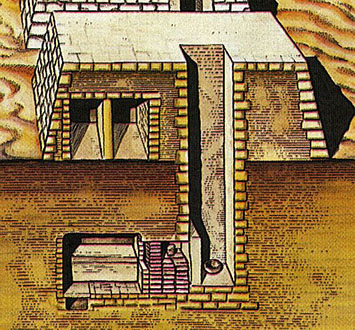
\includegraphics[width=1.0\linewidth]{01/masztaba}
	}
\end{wrapfigure}

\paragraph{1. Masztabák} 
A korai időszakban az uralkodók ún. masztabákba temetkeztek. Ezek a föld alatt lévő sírkamra fölé kerültek, lapos, négyzet alaprajzú, csonkagúla alakú, gyakran egyetlen kőtömbből álló építmények voltak. Masztabák az Óbirodalom idején is készültek, ekkor azonban már nem az uralkodó, hanem a vezír-réteg, vagy a fáraó-feleségek temetkeztek ilyen sírokba.

\begin{wrapfigure}{r}{0.35\textwidth}
	\tcbox[colback=darkgray!85!black,
	left=0mm,right=0mm,top=0mm,bottom=0mm,boxsep=1mm,toptitle=0.5mm,bottomtitle=0.5mm,
	title=\centering{Dzsószer fáraó lépcsős piramisa Szakkarában}]{
		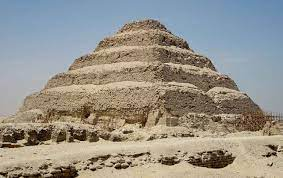
\includegraphics[width=1.0\linewidth]{01/dzsoszer_piramis}
	}
\end{wrapfigure}

\paragraph{2. Lépcsős piramis}
Az Óbirodalom idején az uralkodó megnövekedett tekintélyét, isteni voltát kifejezendő, a lapos masztabák tetejére további szűkebb négyzet-alaprajzú csonkagúlákat helyeztek, hogy magasságát növeljék. Pl.: Dzsószer fáraó lépcsős piramisa Szakkarában.

Dzsószer fáraó piramisa a lépcsős piramisok első példája volt, tulajdonképpen több, egyre kisebb, egymásra rakott masztaba. Szakkarában (a mai Kairótól kb.20 km-re délebbre) található. Kb. 60 m magas, fél-egy méter magasságú mészkőtömbökből épült fel. Alkotója Dzsószer legelső vezírje, papja, orvosa, építésze: Imhotep volt.

\begin{wrapfigure}{r}{0.35\textwidth}
	\tcbox[colback=darkgray!85!black,
	left=0mm,right=0mm,top=0mm,bottom=0mm,boxsep=1mm,toptitle=0.5mm,bottomtitle=0.5mm,
	title=\centering{Sznofru fáraó dahsúri tört falú piramisa}]{
		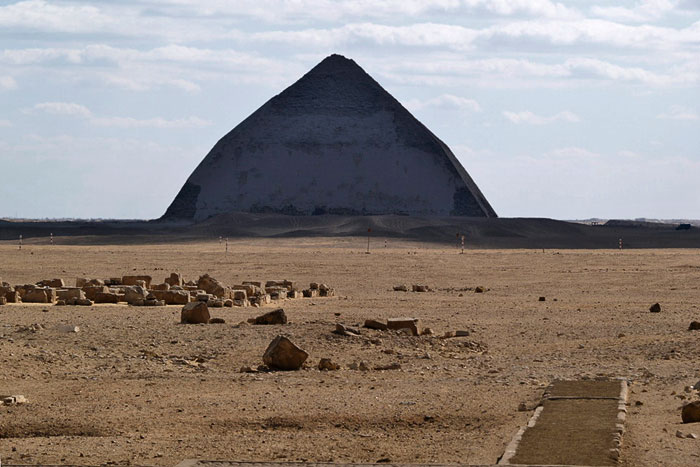
\includegraphics[width=1.0\linewidth]{01/dashur_piramis}
	}
\end{wrapfigure}

\paragraph{3. Tört élű piramis}
Ez az időszak a hatalmas méretű gúla alakzat felépítésének kísérleti szakasza volt. Pl.:t ört élű és tág szögű piramisok Dahsúrban.
A Dzsószer után uralkodó fáraó (Sznefer) már a sok, kis lépcsőfokokból álló gúlaformát próbálta felépíteni. Piramisát azonban homok-alapra építette, és az építkezés közben a kőtömeg alatt megsűllyedt a talaj, a piramis éleinek szögét ezért beljebb kellett dönteni, hogy az építmény alacsonyabb, ezéltal kisebb tömegű legyen. Ennek eredménye lett a dahsúri Tört élű piramis.
A Tört élű piramis közvetlen szomszédságában Sznefer építészei - valószínű, hogy kijavítsák a hibájukat - a Tört élű piramis építésének második szakaszában alkalmazott dőlésszöggel építettek fel egy másik, már valóban a híres gúla-formát mutató sírépítményt, amit a vörös színű mészkövei miatt Vörös piramisnak neveznek.


\paragraph{4. Gúla forma}
\subparagraph{A gúla forma szimbolikája}
A cél elsősorban a magasság növelése volt, hiszen az a fáraó jelentőségét fejezte ki. Másrészt a forma iránti rokonszenv oka az volt, hogy az egyiptomi hitvilágban a gúla-forma több szimbolikus jelentést hordozott. Az egyiptomi teremtés-mítosz ilyennek írta le az ősvízből kiemelkedő őshalmot, azaz az első szárazföldet. A lépcsőzetesség kifejezte a napistenhez, Réhez vezető utat, amin a fáraó szellemi lelke felment az egekbe. A forma hasonló volt a fentről szétágazó nap sugaraihoz, azaz kifejezte Ré, a napisten védelmét az eltemetett fáraó felett. Továbbá minden ősi civilizáció szakrális épülete négyszög alaprajzra kerülő toronyszerű építmény volt - lásd a mezopotámiai zikkuratokat, vagy a maják amerikai templomait, amik hasonló formájúak. A piramis-forma kialakulásának is fontos feltétele volt, hogy ez a forma volt statikailag a legjobban megoldható az ókorban.

\subparagraph{A forma} Az építmény a tökéletességet tükröző szabályos gúla formájú: négyzet alaprajz, amihez minden oldalról a négyzet oldalaival egyenlő hosszúságú oldalú, szabályos háromszögek kapcsolódnak.

\subparagraph{A Gízai piramis-együttes}
Egyiptom legnagyobb piramisát a legidősebb fáraó, Kheopsz építtette (kb.Kr.e.2570-től). Az építkezés több, mint húsz évig tartott, már a fáraó megkoronázásakor elkezdték. A piramis 146m magas (2,3 millió mészkőtömbből építették, amik egyenként másfél méter magas és egy-két méter széles faragott téglatestek, és kb. két és fél tonnát nyomnak).

\begin{wrapfigure}{r}{0.5\textwidth}
	\tcbox[colback=darkgray!85!black,
	left=0mm,right=0mm,top=0mm,bottom=0mm,boxsep=1mm,toptitle=0.5mm,bottomtitle=0.5mm,
	title=\centering{Gízai piramisok}]{
		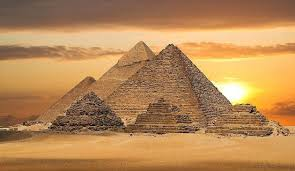
\includegraphics[width=1.0\linewidth]{01/gizai_piramisok}
	}
\end{wrapfigure}

Kheposz piramisa mellett három kisebb piramis is áll, amelyeket felesége és lánytestvérei számára építtetett.
Kheposz fia, Kefrén építette a kissé délebbre álló piramist, ami a fotókon középen áll, és
a három sír-építmény közül a legmagasabbnak tűnik. Ennek csak az az oka, hogy a Kheopsz-piramis szintben lejjebb áll. (Kefrén piramisa 136 m magas.) Az egyetlen, amin fennmaradtak azok a mészkőlapok, amelyekkel
4
ezeket a piramisokat lefedték, hogy a lépcsőzetességet teljesen megszüntetve a sima felületű, (egy hatalmas kristály hatását keltő) szabályos gúlaformát létrehozzák.
A harmadik, még délebbe álló piramis Mükerinosz fáraóé, a legkisebb a trióból, 62m magas.

\subsubsection*{Halotti templomok}

A piramisok mellett halotti templomokat is építettek, ahol a fáraó múmiáját készítették el, illetve a halálával istenné vált fáraónak szentelt templomok szerepét töltötték be az épületek, ahol a fáraó szellemi lelkének áldoztak. Ezek a templomok igen romos állapotban maradtak fenn, a legjobb állapotban megmaradt templom Kefrén fáraóé.

\paragraph{Kefrén halotti temploma Gízában}
A templom Kefrén piramisa előtt áll, mögötte található a Szfinx, így a piramis, a Szfinx és a templom egy tengelyt alkot. A templom hatalmas gránittömbökből épült. Fő részét az a folyosó jelenti, amin a fáraó múmiáját szállították végig. A folyosó két oldalán az istenek szobrai álltak, amiket az ablakokon beeső fény világított meg.

\subsubsection*{Fáraó szobrok}

A fáraó a politika és a vallás feje volt egy személyben. A fáraó szó arab, eredetileg a memphiszi palotát és a palotaőrséget jelentette.

\paragraph{A fáraó uralkodói jelvényei}

	\begin{compactitem}
		\item \underline{Kettős korona:}\\
		Alsó és Felső Egyiptom feletti hatalom szimbóluma. Felső Egyiptomé a fehér - valószínű, hogy ezüstből készült - korona, ami egy csúcsos hegyes sisak volt. Alsó Egyiptomé a piros korona hátul hosszú nyúlvánnyal, elől fémszállal, a homlokán a két terület istenségeinek szimbólumaival, a kobrával és a keselyűvel.
		
		\item \underline{Menész:} a nehéz kettős koronát helyettesítő vászonkendő.
		
		\item \underline{Álszakáll:} bölcsesség, a bölcs uralkodó jelképe.
		
		\item \underline{Pásztorbot alakú jogar:} a népét védelmező uralkodó.
		
		\item \underline{Légycsapó vagy ostor:} az ellenségeit kíméletlenül leigázó uralkodó.
		
		\item \underline{Állatfarok:} a köténye felső részéről lógott le, a harci ügyességekben járatos uralkodó szimbóluma.
	\end{compactitem}

\begin{figure}[H]
	\centering
	\begin{minipage}{0.44\textwidth}
		\begin{tcolorbox}[enhanced,colframe=gray!50!white,
			colbacktitle=gray!15!white,
			coltitle=gray!50!black,
			borderline={0.5mm}{0mm}{gray!15!white},
			borderline={0.5mm}{0mm}{gray!50!white,dashed},
			attach boxed title to top center={yshift=-2mm},
			boxed title style={boxrule=0.4pt},
			title=Kettős korona]{
				
\includegraphics[width=1.0\linewidth]{images/01/kettos_korona}}
		\end{tcolorbox}
	\end{minipage}
	\hfill
	\begin{minipage}{0.44\textwidth}
		\begin{tcolorbox}[enhanced,colframe=gray!50!white,
			colbacktitle=gray!15!white,
			coltitle=gray!50!black,
			borderline={0.5mm}{0mm}{gray!15!white},
			borderline={0.5mm}{0mm}{gray!50!white,dashed},
			attach boxed title to top center={yshift=-2mm},
			boxed title style={boxrule=0.4pt},
			title=Pásztorbot és korbács]{
				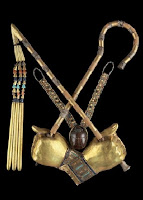
\includegraphics[width=1.0\linewidth]{images/01/pasztorbot_korbacs}}
		\end{tcolorbox}
	\end{minipage}
	\captionsetup{labelformat=empty}
	\caption{}
\end{figure}

\paragraph{A fáraó szobrok rendeltetése}
A fáraók szobrai nem a piramisokban álltak, hanem általában a piramisok mellett lévő halotti templomokban kaptak helyet fülkékben. Nem körüljárhatók, a hátuk gyakran egy laphoz támaszkodik, a figurák szigorúan főnézetre komponáltak.

\begin{wrapfigure}{r}{0.5\textwidth}
	\begin{tcolorbox}[enhanced,colframe=gray!50!white,
		colbacktitle=gray!15!white,
		coltitle=gray!50!black,
		borderline={0.5mm}{0mm}{gray!15!white},
		borderline={0.5mm}{0mm}{gray!50!white,dashed},
		attach boxed title to top center={yshift=-2mm},
		boxed title style={boxrule=0.4pt},
		title=Kefrén fáraó szobra]{
			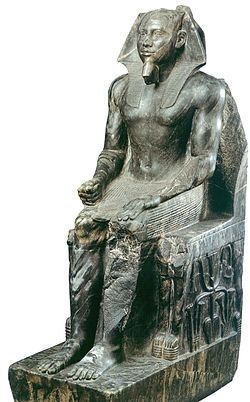
\includegraphics[width=1.0\linewidth]{images/01/kefren_szobra}}
	\end{tcolorbox}
\end{wrapfigure} 

A fáraó-szobor a fáraó halála után egykori ideális testének helyettesítője volt, a visszatérő szellemi lélek számára készítették. Ez volt a jelzés, hogy a lélek tudja, hogy kinek a teste van a templom melletti piramisban. A szobron található ún. kartus - a fáraó nevét tartalmazó ovális alakú jelzés - tájékoztatott a szobor kilétéről. Mivel a visszatérés idejét nem lehetett tudni, a szobornak az örökkévalóságig fenn kellett maradnia, ezért tartós, kemény kőből, a legjobb esteben gránitból készítették. (Ezt délről szállították a Nílus deltájához.)

\paragraph{A fáraószobrok stílus-jellemzői}

A szobor egyben kifejezte azt is, hogy a fáraó halálával istenné vált, így a szobor stílusának minden eleme az isteni tökéletességet kívánja tükrözni.

A fáraóról nem portrét készítettek, hanem a fáraót, mint ereje teljében lévő, kiegyensúlyozott, bölcs, fiatal és szép, azaz ideális és isteni uralkodót örökítették meg a szobrok: nyugodt, mozdulatlan testtartás, frontális beállítás (= minden testrésze a nézővel szembe néz: sem a fej, sem a törzs, sem a lábak nem fordulnak el).

Bal lába mindig előrébb helyezett (de nem lép, mozdulatlan). Magyarázatként szolgálhat erre a testtartásra az, hogy a halálakor a fáraó ezzel fejezte ki az istenek előtt az alázatát, bűnösségét: a szívének volt szüksége támasztásra, ezért kerül mindig a bal láb előbbre.

A tömegkezelés zárt, a szobor egésze tömbszerű, a figura szorosan a combjai mellett tartja a kezét. 

Mereven előrenéző, eszményített arc és tekintet, nyugodt, érzelemmentes, ráncmentes, idealizált, fiatal arc, a fejen általában a menész-korona a kobrával és keselyűvel (Alsó- és Felső-Egyiptom isteneinek szimbólumai, itt azt fejezik ki, hogy ők védelmezik az uralkodó hatalmát a két terület felett).

Az izmokat nem túlhangsúlyozó, finoman, visszafogottan izmos, idealizáló mezítelen felsőtest, egyszerű szoknya.

A kezek ökölbe szorulnak, amiben általában a túlvilági élet kulcsa vagy templomi csörgő van. 

A fáraó-szobrok az Óbirodalom idején általában életnagyságúak, a későbbi korokban méreteik a lehetőségekhez mérten megnőnek, a fáraó nagyságát fejezik ki. (Pl. a Memnón kolosszusok 25 m magasak.)

\paragraph{Híres fáraó szobrok}

	\subparagraph{Dzsószer ülő szobra}
	
	\begin{wrapfigure}{r}{0.45\textwidth}
		\begin{tcolorbox}[enhanced,colframe=gray!50!white,
			colbacktitle=gray!15!white,
			coltitle=gray!50!black,
			borderline={0.5mm}{0mm}{gray!15!white},
			borderline={0.5mm}{0mm}{gray!50!white,dashed},
			attach boxed title to top center={yshift=-2mm},
			boxed title style={boxrule=0.4pt},
			title=Dzsószer szobra eredeti helyén]{
			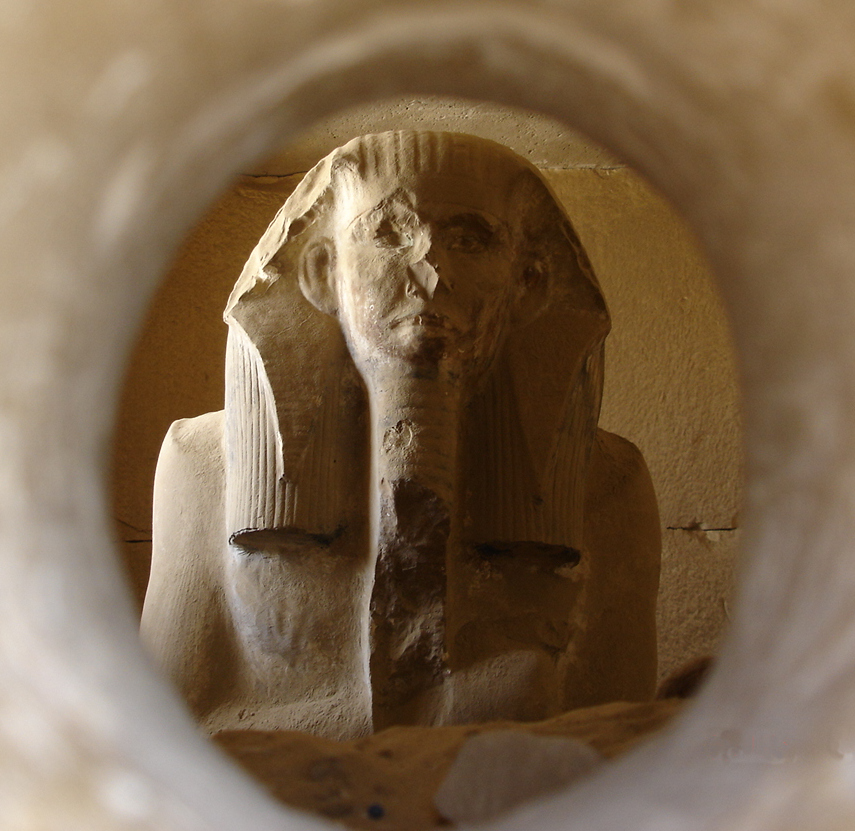
\includegraphics[width=1.0\linewidth]{01/dzsoszer_szobor}}
		\end{tcolorbox}
	\end{wrapfigure} 

	Az egyik legkorábbi fáraószobor. Eredetileg nem a halotti templomban, hanem a lépcsős piramis mellett állt egy befalazott fülke mögött, amin két kis lyuk volt. Egyrészt a visszatérő lélek számára, hogy láthassa, kinek a teste található az itt lévő sírban, másrészt a fáraó számára, hogy láthassa a számára rendezett ünnepségeket.
	
	\subparagraph{Kefrén ülő szobra}
	Dzsószer szobrához hasonlóan kocka alakú trónuson jelenik meg a fáraó. A zárt tömegű, oroszlánlábakkal rendelkező trónus az ország hosszú időn át folyamatos stabilitásának és egységességének kifejezője volt, melyen a fáraó biztos tartással ül. A fáraó fejét hátulról egy sólyom öleli át, ez Hórusz isten, és a fáraó emberi és isteni voltára utal. A szobrot Kefrén halotti templomában találták.
	
	\subparagraph{Mükerinosz triásza}
	Mükerinosz fáraó előszeretettel ábrázoltatta magát a feleségével és nőistenekkel, hogy magát és családját az istenek szférájába tartozóként mutassa be. Ezt fejezi ki az ilyen páros vagy hármas szobrok átölelő mozdulata, ami inkább csak jelzés szerű, hogy a szobor merevségét, földöntúli mozdulatlanságát semmilyen valós mozgás ne törje meg.
	
	\begin{wrapfigure}{r}{0.45\textwidth}
		\begin{tcolorbox}[enhanced,colframe=gray!50!white,
			colbacktitle=gray!15!white,
			coltitle=gray!50!black,
			borderline={0.5mm}{0mm}{gray!15!white},
			borderline={0.5mm}{0mm}{gray!50!white,dashed},
			attach boxed title to top center={yshift=-2mm},
			boxed title style={boxrule=0.4pt},
			title=Mükerinosz triásza]{
				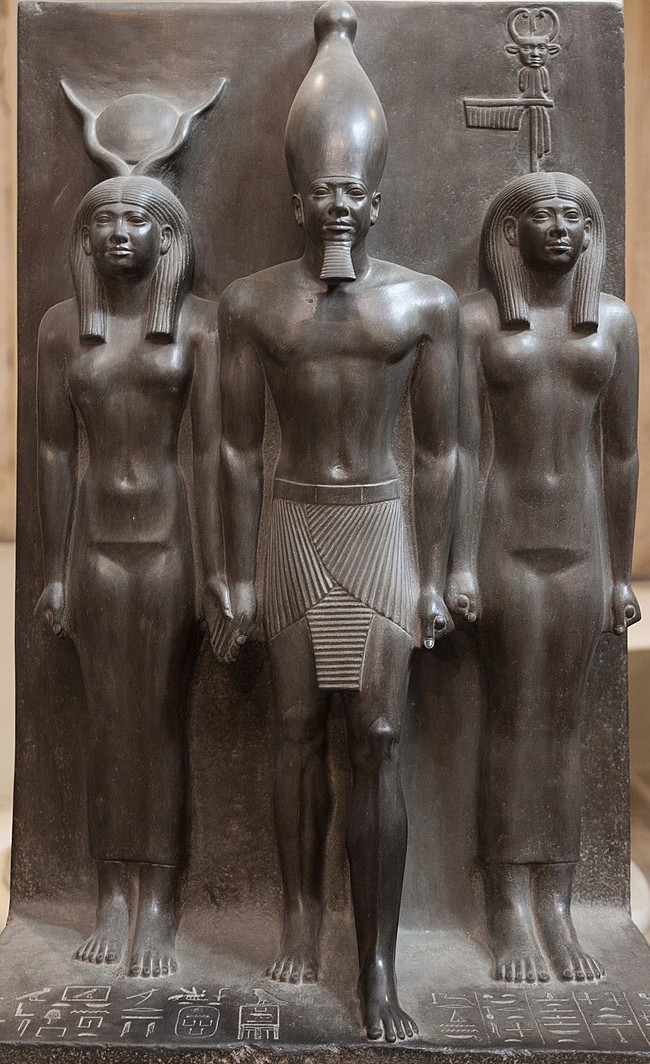
\includegraphics[width=1.0\linewidth]{01/mukerinosz_triasza}}
		\end{tcolorbox}
	\end{wrapfigure} 
	
	Ezeken a szobrokon figyelhető meg a női test sajátos, egyiptomi ábrázolásmódja: a nő-figurát ruha fedi, ám annak általában csak az alsó szegélye látszik, a ruha szorosan a tesre tapad a testformák, tömegek domborulatait finoman sejtetve.
	
	A szoborcsoportban Mükerinosz Hathor (balra) és Anput (jobbra) istennők társaságában van megmintázva.
	
	\subparagraph{Gízai Szfinx}
	A Szfinxet Kefrén fáraóval azonosítják, minthogy az a Kefrén-piramis tengelyében áll. A Gízai Szfinx az egyiptomi művészet legnagyobb szobra: 57 m hosszú és kb. 30 m magas. A helyén álló természetes sziklából faragták ki.
	
	A Szfinx nevet az antik görögök adták a monumentális szobornak, a szinfx ugyanis egy görög mitologikus lény, akinek oroszlán teste és nő-feje van, és megeszi azokat, akik nem tudnak válaszolni a kérdéseire.
	
	A gízai Szfinxet a kincsekkel teli piramis védelmére készítették, és sok írásos szöveg maradt fenn arról, hogy valóban féltek tőle. Az oroszlán testtel ábrázolt fáraó mindig az erős, félelmet keltő, teljhatalmat birtokló uralkodót kívánja a néző elé állítani. A fejen mindig megtalálhtók az uralkodói jelvények, az álszakáll, a menész-koroma, a kobra és a keselyű. A Gízai Szfinx fején is volt álszakáll, ennek egy darabját a 19.sz-ban kiásták, és ma a londoni British Múzeumban őrzik. A figura orrát bizonyos források szerint valamikor a 11-15.század között verték le, de olyan elképzelések is vannak, hogy Napóleon lövette le az ágyúival, amikor a monumentális szobortól félve 30 napig ostromolta azt.
	
	\begin{figure}[H]
		\centering
		\tcbox[colback=gray!85!black,
		left=0mm,right=0mm,top=0mm,bottom=0mm,boxsep=1mm,toptitle=0.5mm,bottomtitle=0.5mm,
		title=\centering{Gízai szfinx}]{
			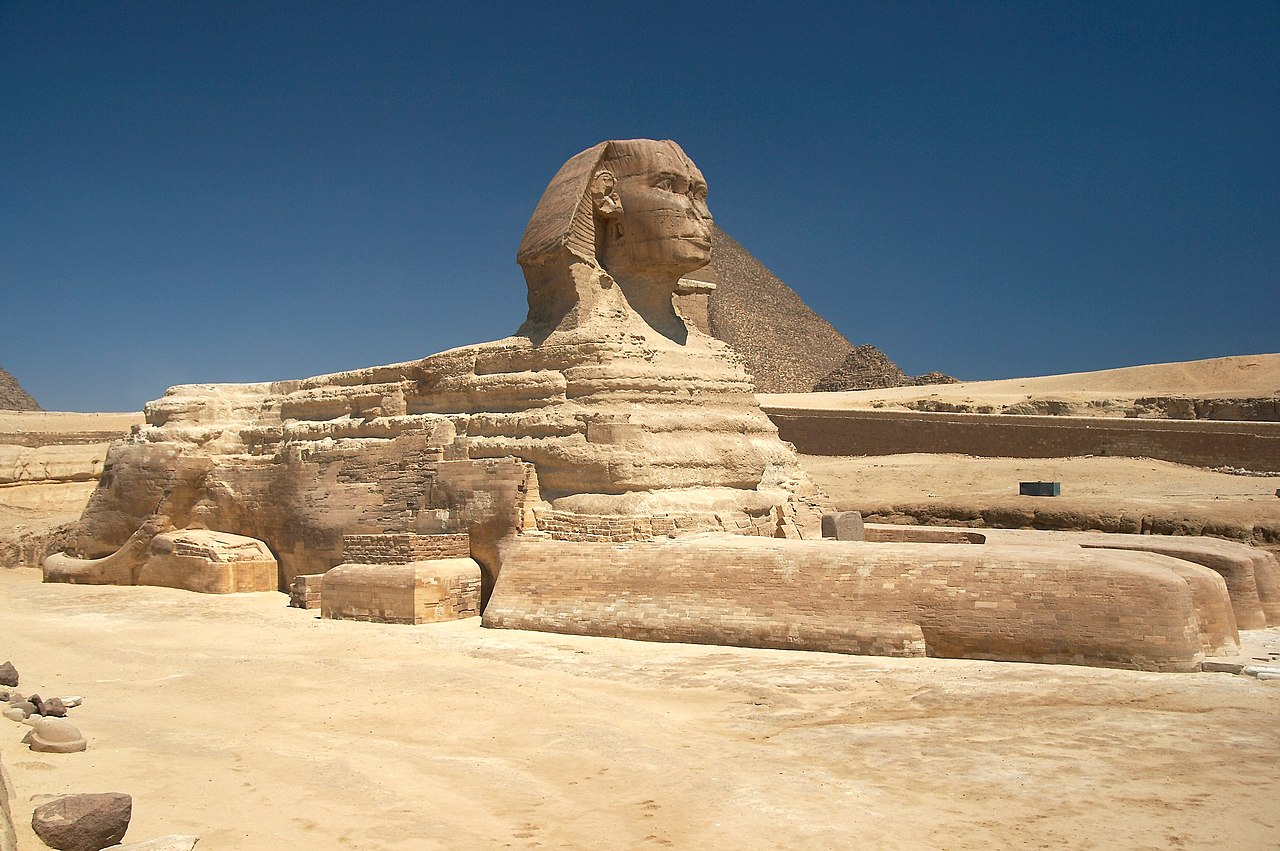
\includegraphics[width=0.9\linewidth]{images/01/szfinx}}
		\captionsetup{labelformat=empty}
		\caption{}
	\end{figure}
	
\subsubsection*{Hivatalnok szobrok}

\paragraph{Kik voltak a vezírek?}
A közigazgatásban részt vevő hivatalnokok, arisztokrata réteg, közvetlenül a fáraó alatti méltóságok viselői (Egyiptom 42 kerületre volt osztva, melynek élén a vezírek álltak) - bírák, hivatalnokok, írnokok, papok, orvosok, építészek, kincstárnokok.

A piramisok belsejével ellentétben a vezírek masztabáinak belső díszítései jobb állapotban maradtak fenn. Megmaradt számos sír dombormű-dísze és szobrászati dísze. A leggyakoribb szobrok az írnokszobrok, de papok és hercegi párok szobrait is ismerjük. Ezeket a szobrokat az idealisztikus, isteni tökéletességet tükröző fáraó-ábrázolásokkal szemben reálisabb megfogalmazásmód, portrészerűség jellemzi, hiszen az ő esetükben nem beszélhetünk istenné válásról a halál után. A szobrok kevésbé tartós anyagokból, puhább kövekből vagy fából készültek.

\begin{wrapfigure}{r}{0.3\textwidth}
	\begin{minipage}{0.3\textwidth}
		\begin{tcolorbox}[enhanced,colframe=gray!50!white,
			colbacktitle=gray!15!white,
			coltitle=gray!50!black,
			borderline={0.5mm}{0mm}{gray!15!white},
			borderline={0.5mm}{0mm}{gray!50!white,dashed},
			attach boxed title to top center={yshift=-2mm},
			boxed title style={boxrule=0.4pt},
			title=Ülő írnok szobra]{
				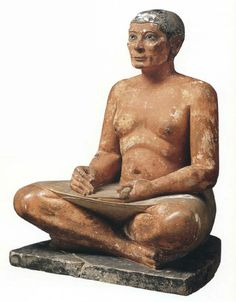
\includegraphics[width=1.0\linewidth]{01/irnok_szobor}}
		\end{tcolorbox}
	\end{minipage}
	\begin{minipage}{0.3\textwidth}
		\begin{tcolorbox}[enhanced,colframe=gray!50!white,
			colbacktitle=gray!15!white,
			coltitle=gray!50!black,
			borderline={0.5mm}{0mm}{gray!15!white},
			borderline={0.5mm}{0mm}{gray!50!white,dashed},
			attach boxed title to top center={yshift=-2mm},
			boxed title style={boxrule=0.4pt},
			title=Falusi bíró szobra]{
				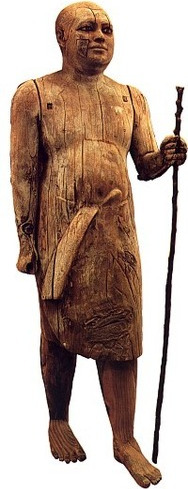
\includegraphics[width=1.0\linewidth]{01/falusi_biro}}
		\end{tcolorbox}
	\end{minipage}
	\begin{minipage}{0.3\textwidth}
		\begin{tcolorbox}[enhanced,colframe=gray!50!white,
			colbacktitle=gray!15!white,
			coltitle=gray!50!black,
			borderline={0.5mm}{0mm}{gray!15!white},
			borderline={0.5mm}{0mm}{gray!50!white,dashed},
			attach boxed title to top center={yshift=-2mm},
			boxed title style={boxrule=0.4pt},
			title=Rahotep \& Nofret]{
				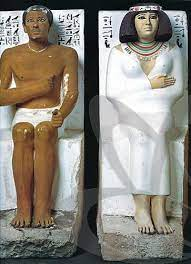
\includegraphics[width=1.0\linewidth]{01/rahotep_nofret}}
		\end{tcolorbox}
	\end{minipage}
\end{wrapfigure} 

\paragraph{Louvre-i írnok szobra}
A szobrot Szakkarában találták, ma Párizsban, a Louvre-ban található. Bár a figura itt is merev főnézetre komponált, az írnokot a művész életének szokásos jelentében ábrázolja: munkavégzés közben, életszerű testtartásban. Törökülésben, ölében papirusztekerccsel, írószerszámmal a kezében. 

Arca portrészerű: a szobornak nem célja, hogy az ábrázoltat megszépítse, a valós modell sajátos vonásait mutatja be. A figura állkapocscsontja széles, homloka, álla alacsony, szája sajátosan keskény és széles, fülei nagyok, teste sem fiatalos szépséget, hanem plöttyhedt melleket, pókhasat mutat.

\paragraph{Falusi bíró}
Nevét úgy kapta, hogy a szobrot megtaláló munkásokat saját falujuk bírójára emlékeztette, az ábrázolt szemlély azoban valójában egy pap volt. A szobor különlegessége, hogy fából van. Stílusára ugyanaz a realizmus jellemző, ami a louvre-i írnokszobron mutatkozott meg: a pap - noha főnézetre komponált, és bal lábát a fáraószobrokhoz hasonlóan előbbre helyezi - egy jóltáplált, kövérkés ember volt, kerekded fejjel, tokás nyakkal, vastag lábszárakkal, pocakkal. (112 cm) 

\paragraph{Rahotep és Nofret}
A hercegi pár csoportjának komponálásmódja igazodik a fáraó-ábrázolásokhoz: főnézetre komponáltak, frontális beállításúak, zárt négyzetes székeken ülnek, zárt a tömegkezelésük, merev tekintetük van, a nőalak testre simuló ruházzattal ábrázolt, arcukon mégis - különösen a nőjén - a valósághűségre való törekvés érvényesül.

\subsubsection*{A dombormű-szobrászat}

Az Óbirodalom domborművei a hivatalnokok masztabáiban maradtak fenn.

Ezek lapos domborművek voltak (a figurák kevéssé emelkednek ki a falból), és festetve voltak.

Témáik egyrészt az elhunyt és családjának hétköznapjait mutatták be, a mindennapi feladatok és munkavégzés közben ábrázolták őket és házuk népét. Vetés, aratás, háziállatok leölése, adminisztráció közben, gyakran a halott életrajzát is megfestették. 

A domborművek másik témaköre a halál utáni élethez szükséges élelem és eszközök felvonultatása volt. Több falat is szántak az áladozati ajándékok ábrázolására.

A domborművek stílusát a legnagyobb felületek törvénye határozta meg: az adott testrészt az arra leginkább jellemző nézetből ábrázolták. A fejet oldalról, a szemet szemből, a törzset, vállakat szemből, a melleket oldalról, a kezeket, csípőt, lábakat ismét oldalról. Ugyanez a törvény érvényesült a tárgyak ábrázolásánál: egy asztal megfogalmazásánál például az asztal lábát oldalról festették meg, az asztallapot azonban felülnézetből, miközben az ezen elhelyezkedő tárgyakat ismét oldalról, így azok olyan hatást keltenek, mintha egymásra lennének helyezve.

A figurák egymáshoz viszonyított arányaiban is az ókori kultúrákban elterjedt hagyomány tapasztalható: a figura mérete a rangját fejezi ki, mennél nagyobb az alak, annál jelentősebb személy a kompozícióban.

\begin{figure}[H]
	\begin{tcolorbox}[enhanced,colframe=gray!50!white,
		colbacktitle=gray!15!white,
		coltitle=gray!50!black,
		borderline={0.5mm}{0mm}{gray!15!white},
		borderline={0.5mm}{0mm}{gray!50!white,dashed},
		attach boxed title to top center={yshift=-2mm},
		boxed title style={boxrule=0.4pt},
		title=Domborművek hivatalnokok masztabáiból]{
		\begin{minipage}{0.33\textwidth}
					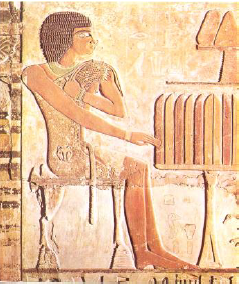
\includegraphics[width=1.0\linewidth]{01/dombormu1}
		\end{minipage}
		\hfill
		\begin{minipage}{0.25\textwidth}
					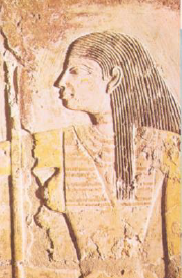
\includegraphics[width=1.0\linewidth]{01/dombormu2}
		\end{minipage}	
		\hfill
		\begin{minipage}{0.36\textwidth}
			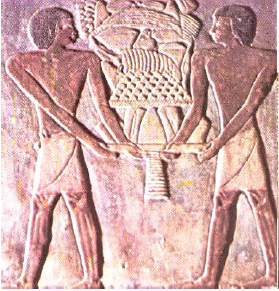
\includegraphics[width=1.0\linewidth]{01/dombormu3}
		\end{minipage}}
	\end{tcolorbox}
\end{figure}

\cleardoublepage

\subsection*{A Közép. és Újbirodalom művészete}

\subsubsection*{A Középbirodalom történelmi háttére (kb. Kr. e. 2000-1700)}

Kr.e. 2000 táján meggyengült a fáraók hatalma, Egyiptom kisebb részekre szakadt szét, ahol a vezírek kiskirályokként uralkodtak. Súlyosbította a helyzetet, hogy délen nomád bevándorló népek végeztek hatalmas pusztítást. Erre az átmeneti időszakra a zűrzavar, éhezés, fosztogatás volt jellemző - az óbirodalmi királysírokat, a piramisokat már ekkor kirabolták.

Ebből a zűrzavarból Théba városa emelkedett ki, Délen, ez lett a Középbirodalom központja. A fáraó újra fölállította és irányítása alá vonta a közigazgatási kerületeket, megerősítette, megszilárdította a központi hatalmat. Ettől a korszaktól kezdve nem építettek piramisokat, hanem Théba mellett a Nílus nyugati partján lévő sziklás vidéken sziklasírokba temetkeztek az uralkodók.

\subsubsection*{Az Újbirodalom történelmi háttere (Kr.e. 1600-1000)}

Egy második átmenetileg nem egységes időszak után egy fáraónő, Hatsepszut kezébe került a hatalom, aki számos építkezéssel, hódítással, a kereskedelem fellendítésével írta be magát a történelem könyvébe. Mostohafia III. Thotmesz szintén hadjáratairól ismert. III. Amenhotep jó diplomáciai készségéről, és a mezopotámiai városokkal, népcsoportokkal kötött szövetségeiről, kereskedelmi kapcsolatairól híres. Ő kezdte el a luxori és karnaki templomok építését.

Különleges korszakot képvisel IV.Amenhotep fáraó, aki nevét Ehnatonra változtatva az addigi Amon papságot és Amon kultuszát megszüntette, és egyedüli istennek Aton istent tette meg, akit a Nap, mint égitest istenének tartottak. Így jött létre az Egyiptom történelmében egyedülálló monoteista korszak, amit Amarna-kornak nevezünk. Valószínű, hogy Ehnaton leszármazotta volt Tutanhamon fáraó, aki - amint azt neve is mutatja - visszaállította az Amon-kultuszt. Tutankhamon volt az egyetlen fáraó, akinek sírja érintetelenül megmaradt, és tartalmát hiánytalanul ismeri a régészettudomány.

A korszak következő periódusában ún. katonafáraók uralkodtak: II.Ramszesz, akinek hódításairól számtalan dombormű tanúskodik; Széthi, akik az Egyiptomba betörő népek visszaverésén fáradozott. Az így megteremtett biztonság és béke idejében épültek tovább, és II. Ramszesz dicsőségét hirdették a már említett thébai templomok: a luxori és karnaki templom. Az újbirodalom kora a Ramszeszek uralkodásával ért véget, akiket a megnövekedett hatalmat gyakorló papság döntött le a trónról.

\subsubsection*{A Királyok völgye}

\begin{wrapfigure}{r}{0.5\textwidth}
	\begin{tcolorbox}[enhanced,colframe=gray!50!white,
		colbacktitle=gray!15!white,
		coltitle=gray!50!black,
		borderline={0.5mm}{0mm}{gray!15!white},
		borderline={0.5mm}{0mm}{gray!50!white,dashed},
		attach boxed title to top center={yshift=-2mm},
		boxed title style={boxrule=0.4pt},
		title=Királyok völgye]{
			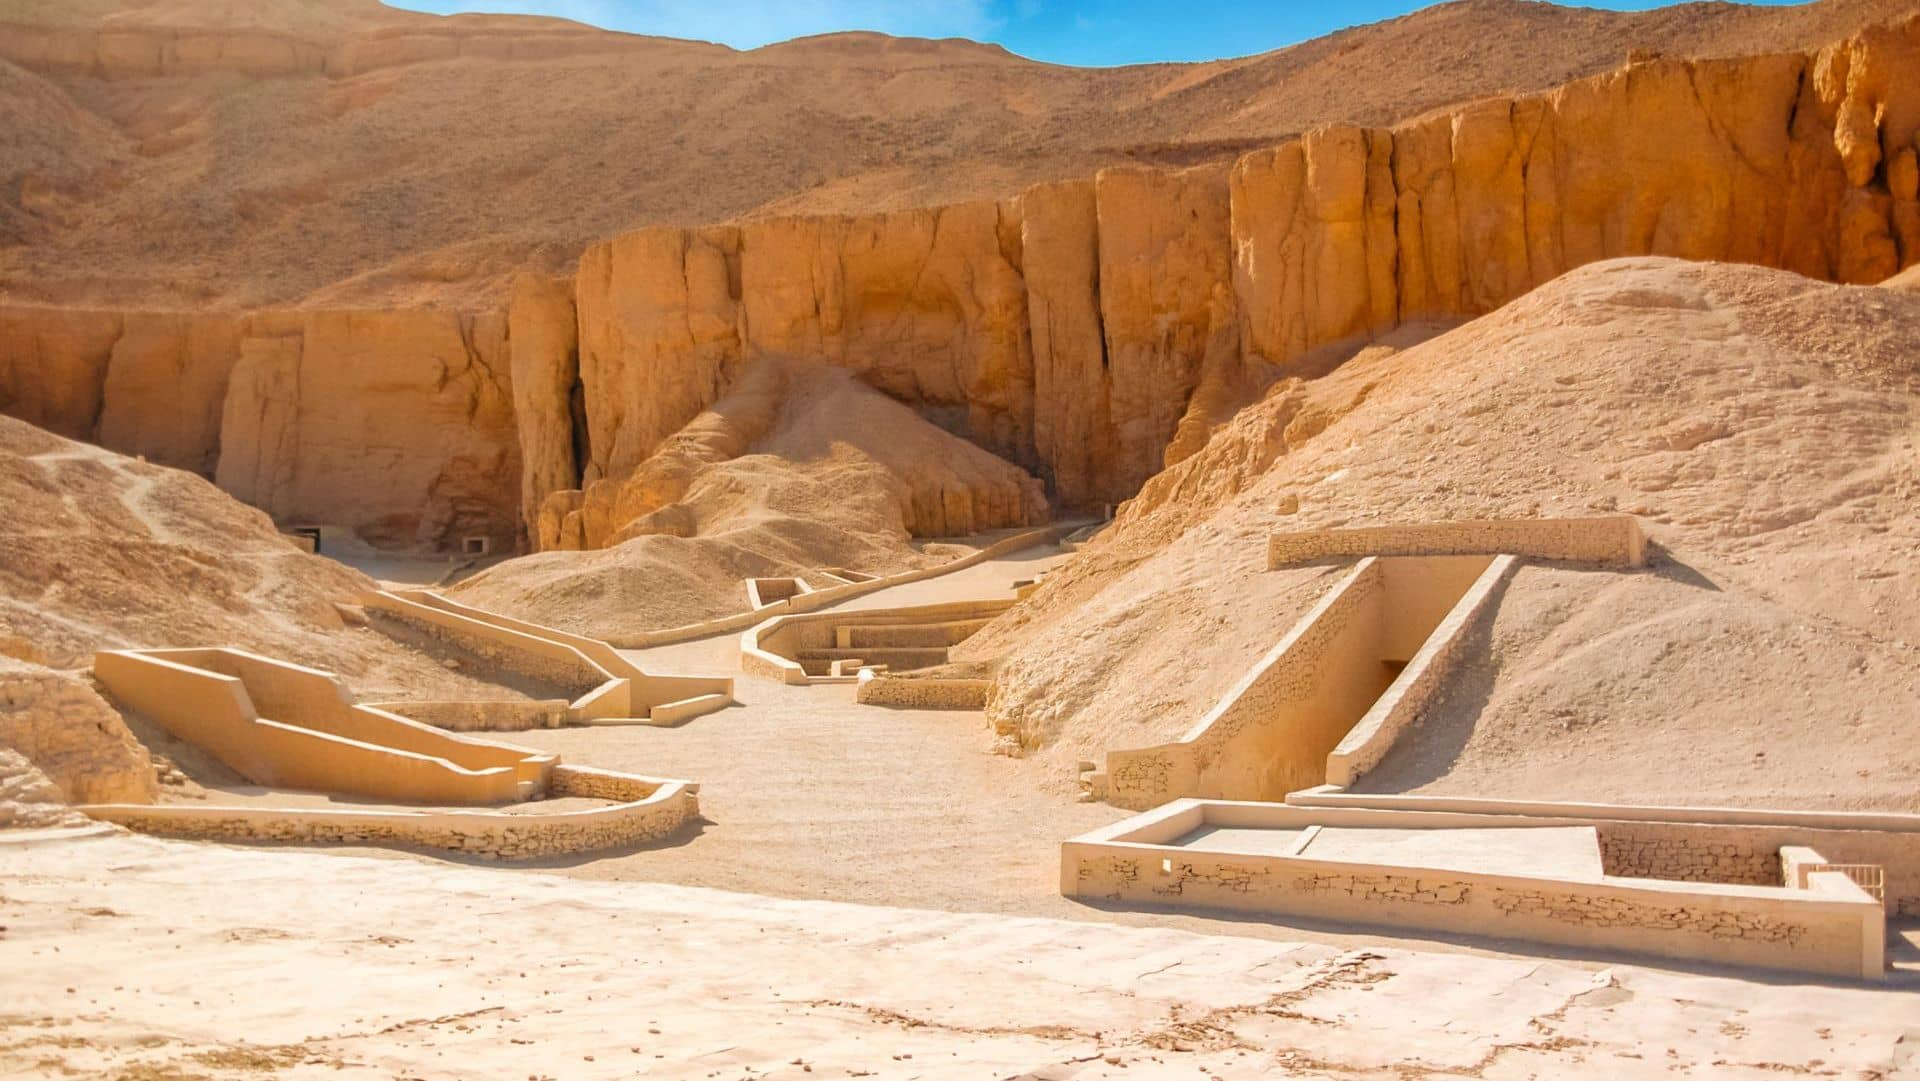
\includegraphics[width=1.0\linewidth]{01/kiralyok_volgye}}
	\end{tcolorbox}
\end{wrapfigure}

\paragraph{Védelem a sírrablóktól} Mivel a piramisokat már az Óbirodalom idején, főleg az első átmeneti kor alatt kifosztották, a Középbirodalomtól kezdve a fáraók múmiája számára nem építettek messziről látható sírépítményeket, hanem inkább a holtest és a sírkincsek elrejtésére törekedtek. A Középbirodalomtól kezdve a fáraók temetkezési helye a Théba várossal (Ma Luxor és Karnak városok találhatók itt, kb. 7oo km-re Kairótól.) szemben lévő sziklás vidék a Nílus nyugati partján, ma ezt Királyok völgyének nevezik.

\paragraph{A természeti adottságok kihasználása}Valószínű, hogy azért is éppen ez a terület vált az Újbirodalom fáraóinak temetkezési helyévé, mert a sírok fölött piramis alakú, természetes sziklák húzódnak. 62 sírt tártak fel eddig a völgyben, bár nem mindegyik volt fáraó-sír.

\begin{wrapfigure}{r}{0.45\textwidth}
	\begin{tcolorbox}[enhanced,colframe=gray!50!white,
		colbacktitle=gray!15!white,
		coltitle=gray!50!black,
		borderline={0.5mm}{0mm}{gray!15!white},
		borderline={0.5mm}{0mm}{gray!50!white,dashed},
		attach boxed title to top center={yshift=-2mm},
		boxed title style={boxrule=0.4pt},
		title=Sziklasír felépítése]{
			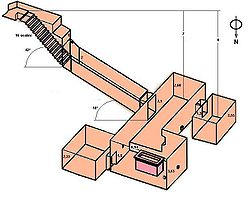
\includegraphics[width=1.0\linewidth]{01/sziklasir_alaprajza}}
	\end{tcolorbox}
\end{wrapfigure}

\paragraph{A sírok felépítése} Több teremből álló, általában észak-déli fekvésű, 2m szélességű folyosók.

A sír néhány lefelé vezető lépcsőfokkal kezdődik, ez után egy hosszú folyosó vezet lefelé, kb. 5 m mélyre. Ennek két oldalán kis termek nyílnak, ahol a fáraónak szánt adományok, áldozati ajándékok kaptak helyet. 

A folyosó végén és a legmélyebben található a sírkamra a fáraó nagyméretű, általában gránitból készült szarkofágjával. A sírkamra mellett egy kincstárszoba is volt a fáraó életében használt személyes tárgyak tárolására.

A hosszan elnyúló folyosót gyakran mély aknák szakítják meg az illetéktelen betolakodók likvidálására, valamint a valódi sírkamra és a kincstár előtt egy-egy festett de üresen hagyott kamrát is kialakítottak, hogy a sírrablók azt higgyék, hogy a sírt már előttük kirabolták.

\begin{wrapfigure}{r}{0.45\textwidth}
	\begin{minipage}{0.45\textwidth}
		\begin{tcolorbox}[enhanced,colframe=gray!50!white,
			colbacktitle=gray!15!white,
			coltitle=gray!50!black,
			borderline={0.5mm}{0mm}{gray!15!white},
			borderline={0.5mm}{0mm}{gray!50!white,dashed},
			attach boxed title to top center={yshift=-2mm},
			boxed title style={boxrule=0.4pt},
			title=Sziklasír belülről]{
				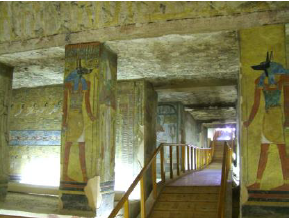
\includegraphics[width=1.0\linewidth]{01/sziklasir}}
		\end{tcolorbox}
	\end{minipage}
	\begin{minipage}{0.45\textwidth}
		\begin{tcolorbox}[enhanced,colframe=gray!50!white,
			colbacktitle=gray!15!white,
			coltitle=gray!50!black,
			borderline={0.5mm}{0mm}{gray!15!white},
			borderline={0.5mm}{0mm}{gray!50!white,dashed},
			attach boxed title to top center={yshift=-2mm},
			boxed title style={boxrule=0.4pt},
			title=Tutanhamon sírkamrája]{
				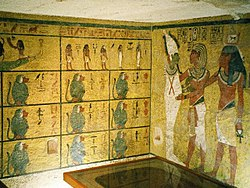
\includegraphics[width=1.0\linewidth]{01/sirkamra_diszites}}
		\end{tcolorbox}
	\end{minipage}
\end{wrapfigure} 

\paragraph{Díszítés}
A sírfolyosók falait az ún. Halottak könyve díszítette domborműveken és festményeken. Ez a fáraó lelkének alvilági utazását beszélte el, ahogyan a különböző istenekkel találkozik, ahogy szívét megmérik, vagy egyéb megpróbáltatásokat áll ki, hogy elnyerje az örök életet.

\paragraph{Tutanhamon fáraó sírja}
A Királyok völgyének leghíresebb sírja Tutanhamón fáraóé. Ez a legkisebb sír a völgyben, mindössze 3 kis helyiségből áll, összesen talán 25 négyzetméter területű. A sír azért különleges, mert ez volt az egyetlen sír, amit még nem raboltak a XX. századra.

\clearpage

\subsection*{Templom építészet}

\paragraph{Funkciója}
A Közép- és Újbirodalom idején a sírépítmények helyett a templomok kapták a fő szerepet, az egyiptomi építészet monumentalizmusa ezekben érvényesült. Ezek a templomok több fáraó uralkodása alatt épültek fel, a fáraó testének mumifikálására is szolgáltak, és a halálával istenné vált fáraó áldozati templomai is voltak egyben.

E mellett új elemként jelentős szerepet kapott bennük az uralkodói reprezentáció. A fáraónak a társadalomban betöltött rangját, nagyságát, dicsőséges isteni voltát, elsődleges szerepét külsőségekkel is érzékeltették. Pompás szertartásokra, felvonulásokra, nagy tömegek befogadására alkalmas tereket alakítottak ki, hatalmas méretű fáraószobrokat és oszlopokat állítottak fel. Az uralkodó hatalmának dicsőítését ábrázoló vagy a fáraó istenné válását bemutató nagyméretű és nagy mennyiségű domborműveket faragtattak.

\paragraph{Alaprajzi elrendezés}

Az újbirodalombeli templomok legfőbb jellemzője az axialitás, azaz a tereknek egyetlen tengelyre való felfűzése (axis = tengely). A különböző terek egymás után sorakozva egy hosszú, elnyúló téglalapot alkotnak, ahol a terek szakralitása, szent volta a térsor végén álló szentély felé egyre inkább fokozódik.

\subparagraph{Szfinxekkel övezett út} A tér-együttes egy úttal kezdődik, aminek két oldalán a fáraó szfinx-szobrai ritmikusan egymás után sorolódva a fáraó hatalmának állandóságát fejezik ki.

\subparagraph{Pülón} A bevonulási út végén egy vastag és magas fal áll, amin a fáraót dicsőítő domborművek kaptak helyet. Ez a fal a templom kapuja, előtte a fáraó nagyméretű szobrai állnak, valamint két gránit-obeliszk. Az obeliszk igen magas, négyszögletű emlékoszlop, négy oldalán a fáraó kilétéről hieroglifákkal írt szöveg, tetején egy hegyes szögű piramidion található az egykori piramisforma maradványaként, annak szimbolikus jelentéseivel is rendelkezve.

\subparagraph{Udvar} négyzet alaprajzú, nagyméretű, fedetlen udvar, négy oldalán általában páros oszlopokkal, az oszlopok közt fáraók és istenek szobraival. Az udvarban a köznép is tartózkodhatott, és látványos szertartások helye volt.

\subparagraph{Hüposztil csarnok} A templomok következő - építészettörténetileg legjelentősebb, a későbbi korok által továbbfejlesztett - tere, oszloposos csarnok. Általában téglalap alaprajzú, fedett tér, ahol a hatalmas oszlopok súlyos gerendákat tartanak. A csarnok középső tere, azaz hajója kiemelkedik a mellette lévők közül, és a kiemelkedő falát ablakokkal törik át a zárt tér megvilágításának érdekében. Az ilyen szerkezeti felépítést és megvilágítási módot bazilikális szerkezetnek nevezzük. Ennek a később igen gyakori szerkezeti megoldásnak legelső példáit láthatjuk az Egyiptomi újbirodalombeli templomokban. Ebben a térben még nagyobb számú tömeg tartózkodhatott, a szertartások azonban intimebbek voltak, mint az udvarban.

\subparagraph{Szentély} A térsor végén található, több kisebb termet, cellát magába foglaló, a templomban a legszentebb tér-együttes. Ezekben a termekben zajlott a mumifikálás, vagy a fáraóknak és más istenek szóló áldozat. Valamint vallásos relikviákat őriztek ezekben a cellákban. Ide már csak a fáraó és a papok léphettek be.

\paragraph{Szerkezet}
Az egyiptomiak nem ismerték a boltívet, a tartó szerepű építészeti elemeik az oszlopok, a teret lefedő szerepű építészeti elemeik a gerendák voltak. Az egyiptomi oszlopok alul egyszerű lábazatot kapnak, felül pedig fejezettel díszítettek, amik az összecsukódott lótusz vagy a szétágazó papiruszvirág formáját idézik. (A lótuszvirág Felső-Egyiptom, a papirusz Alsó-Egyiptom szimbóluma volt.)

\clearpage

\subsubsection*{A leghíresebb templomok az Újbirodalom korából}

\begin{wrapfigure}{r}{0.5\textwidth}
		\tcbox[colback=darkgray!85!black,
		left=0mm,right=0mm,top=0mm,bottom=0mm,boxsep=1mm,toptitle=0.5mm,bottomtitle=0.5mm,
		title=\centering{Luxori templom}]{
				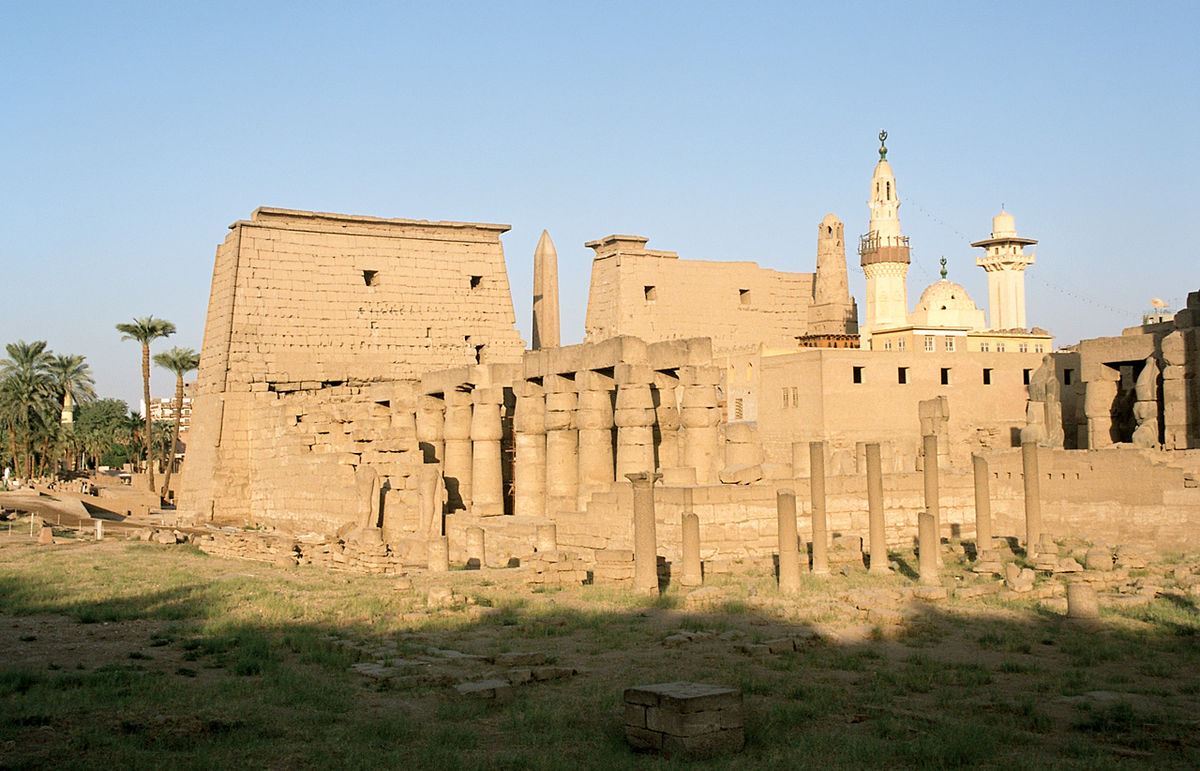
\includegraphics[width=1.0\linewidth]{01/luxori_templom}}
\end{wrapfigure} 

\paragraph{Luxori templom}
A fent leírt alaprajzi formát követi, II. Ramszesz kezdte el építeni, az ő 24 m magas szobrai állnak a pülón előtt. Obeliszkjei közül már csak egy áll itt, a másikat Napóleon Párizsba szállítatta, ma a Place de la Concorde-on áll. A pülón felületét II. Ramszesz hadjáratait dicsőítő vájt domborművek díszítik. Az Újbirodalomban kívül és belül egyaránt vájt domborműveket faragtak: ezek a falfelületbe akár 10 cm mélyen bevésett, nem kidomborodó reliefek voltak. Ennek két oka volt: egyrészt így akarták megvédeni a domborművet a folyamatosan pusztító homoktól, ami lecsiszolta a felületüket, másrészt a következő fáraóktól, akik előszeretettel kaparták le az előző uralkodó kartusát a falakról, és helyettesítették a sajátjukkal.

\paragraph{Karnaki nagy Amon-templom}
Ez a templom a legnagyobb fennmaradt egyiptomi épület: több, mint másfél km hosszú, 10 katedrális férne el benne. Alaprajza szintén a fent leírt rendszert követi, azzal a különbséggel, hogy minden újabb tér előtt egy újabb hatalmas pülón áll, amit más-más fáraó épített. A templomot III. Amenhotep kezdte el építeni, de majdnem 1500 éven keresztül tartott a munka, pontosabban folyamatosan alakították, az újabb fáraók újabb tereket fűztek a már meglévőkhöz. A karnaki templom legjelentősebb tere a 134 oszlopból álló hüposztil csarnok, ami a legnagyobb fedett (kőből) épített tér a művészet történetében: 152 m hosszú, és 52 m széles.

\begin{figure}[H]
	\centering
	\begin{tcolorbox}[enhanced,colframe=gray!50!white,
		colbacktitle=gray!15!white,
		coltitle=gray!50!black,
		borderline={0.5mm}{0mm}{gray!15!white},
		borderline={0.5mm}{0mm}{gray!50!white,dashed},
		attach boxed title to top center={yshift=-2mm},
		boxed title style={boxrule=0.4pt},
		title=Az Amon-Ré templomkörzet]{
			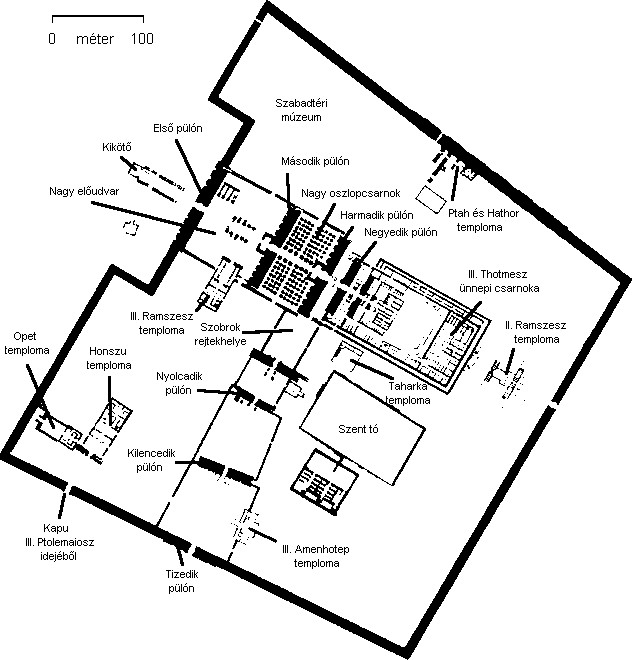
\includegraphics[width=1.0\linewidth]{01/amon_re_templom_alaprajz}}
		
		\tcbox[colback=darkgray!85!black,
		left=0mm,right=0mm,top=0mm,bottom=0mm,boxsep=1mm,toptitle=0.5mm,bottomtitle=0.5mm,
		title=\centering{Amon-Ré templomkörzet a levegőből}]{
			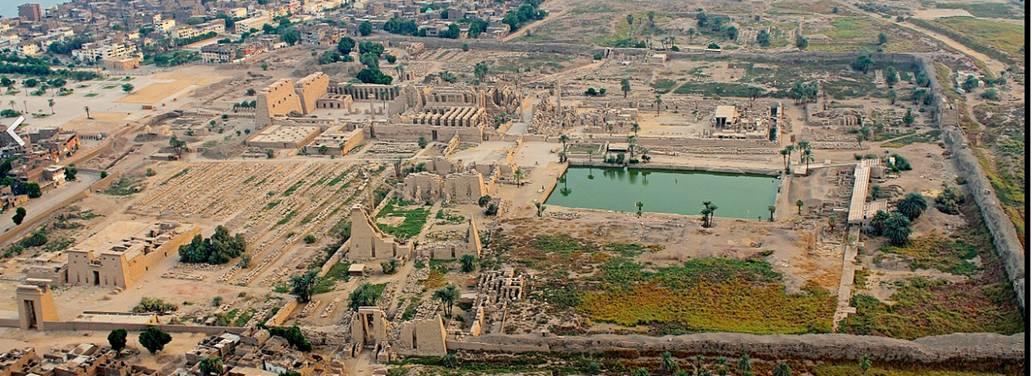
\includegraphics[width=1.0\linewidth]{01/amon_re_templom}}
	\end{tcolorbox}
\end{figure}

\clearpage

\begin{wrapfigure}{r}{0.5\textwidth}
	\tcbox[colback=darkgray!85!black,
	left=0mm,right=0mm,top=0mm,bottom=0mm,boxsep=1mm,toptitle=0.5mm,bottomtitle=0.5mm,
	title=\centering{Memnón-kolosszusok}]{
		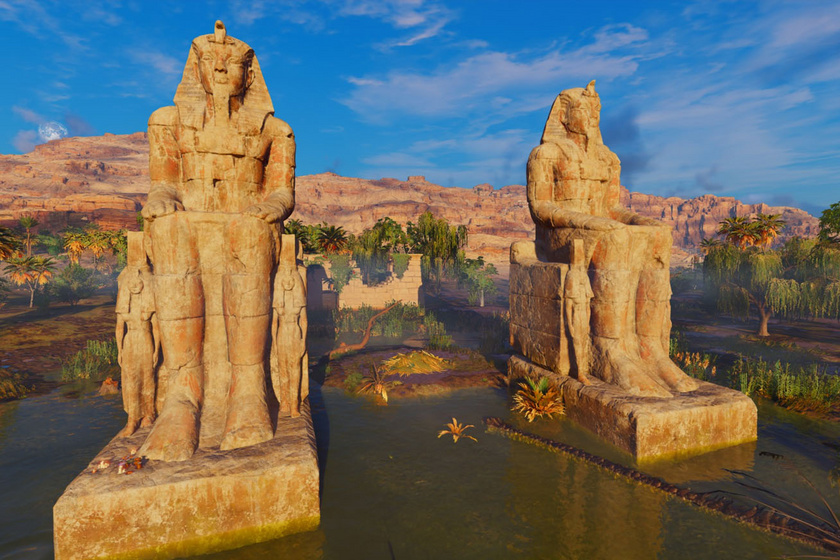
\includegraphics[width=1.0\linewidth]{01/memnon_kolosszusok}}
\end{wrapfigure} 

\paragraph{Memnón-kolosszusok}
A templom a Nílus bal partján volt található, viszonylag közel a folyóhoz. Ez volt a veszte, valamint az, hogy részben szárított agyagtéglából építették. Az áradások során a Nílus elmosta a templomot, csupán a pülónok előtt álló kőből épített/faragott kolosszális méretű, több, mint 25 m magas, III. Amenhotepet - az építtetőt - ábrázoló szobrok maradtak fenn. A szoborkolosszusok a görög trójai mondakör egy alakjáról kapták a nevüket (őket is Hérodotosz, az Egyiptomról először író antik "történész" nevezte el), Memnónról, aki a görög mitológiában sívító hangon üdvözli az anyját. A szobrokon ugyanis számos luk található, az erős szél hatására ezek a lukak sivító hangot adnak ki.

\begin{wrapfigure}{r}{0.5\textwidth}
	\tcbox[colback=darkgray!85!black,
	left=0mm,right=0mm,top=0mm,bottom=0mm,boxsep=1mm,toptitle=0.5mm,bottomtitle=0.5mm,
	title=\centering{Hatsepszut temploma}]{
		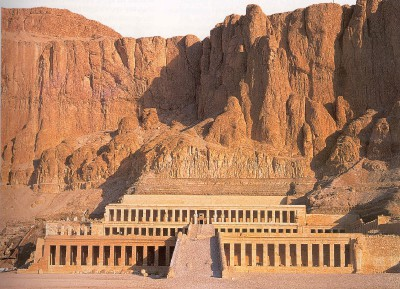
\includegraphics[width=1.0\linewidth]{01/hatsepszut_templom}}
\end{wrapfigure} 

\paragraph{Hatsepszut fáraónő temploma}
Hatszepszut az első Újbirodalombeli fáraók közé tartozott, aki férje halála után átvette a hatalmat. Hatalmas méretű, sajátos felépítésű templomot emelt magának. A templom a Nílus nyugati partján található, közel a Királyok völgyéhez, egy hatalmas sziklaegyütteshez támaszkodva. Az épület különlegessége az, hogy teraszosan épül fel: három, egyre magasabb, a sziklához egyre közelebb álló teraszból áll. Az utolsó teraszról már a szikla belsejébe lehet jutni, ott található a fáraónő szentélye és egyben sírkamrája is.
Hatsepszut - annak ellenére, hogy nő volt - férfiként ábrázoltatta magát szobrain, isteni eredetű ugyanis csak férfi lehetett. Hatsepszut Hathor istennőtől származtatta magát, ezért templomának oszlopain tehénfülű Hathor-fejezetek vannak.

\subsubsection*{Az Amarna-kor művészete}

\begin{wrapfigure}{r}{0.27\textwidth}
	\begin{minipage}{0.27\textwidth}
		\tcbox[colback=darkgray!85!black,
		left=0mm,right=0mm,top=0mm,bottom=0mm,boxsep=1mm,toptitle=0.5mm,bottomtitle=0.5mm,
		title=\centering{Ehnaton szobra}]{
			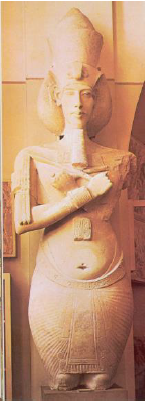
\includegraphics[width=1.0\linewidth]{01/ehnaton}}
	\end{minipage}
	\begin{minipage}{0.27\textwidth}
		\tcbox[colback=darkgray!85!black,
		left=0mm,right=0mm,top=0mm,bottom=0mm,boxsep=1mm,toptitle=0.5mm,bottomtitle=0.5mm,
		title=\centering{Nofertiti büsztje}]{
			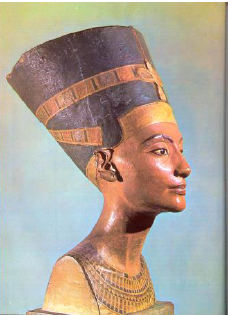
\includegraphics[width=1.0\linewidth]{01/nofertiti}}
	\end{minipage}
\end{wrapfigure} 

Az \textbf{Újbirodalom korának sajátos periódusa} volt Echnaton fáraó korszaka (Kr.e. 1352-1336), amit a fáraó által 15 év alatt felépített új fővárosról, Tell-al-Amaranáról neveztek el.

Echnaton eredti neve IV. Amenhotep volt, de a fáraó teljes mértékben megváltoztatta a vallást: bevezette Aton isten kultuszát, és vele a monoteizmust. Új nevében is Aton isten nevét fedezhetjük fel.
Megváltozik a művészet is: Echnatonnak nem célja, hogy isteni származását bizonyítsa, ő az egyetlen fáraó, aki nem tartotta magát istenségnek. Ezért művészete sem az Óbirodalomban szokásos isteni szépséget kívánja a néző elé állítani.

\paragraph{Ehnaton szobra}
Az uralkodói jelvények követik a korábbi hagyományokat, a részletek azonban eltérnek az előző korok fáraó-ábrázolásaitól: realizmus érzékelhető a stílusban. Sajátos hosszúkás, keskeny arca, keskeny, széles szeme, vékony nyaka, húsos nagy szája, előreugró álla van Echnatonnak. Testfelépítése is egyedi: vékony felsőteste, széles csípője, combjai vannak. Tell-el-Amarnában fennmaradt írások szerint Echnaton beteg volt, ennek volt következménye a sajátos fizikum. (Talán nem véletlen, hogy Echnaton ennyire ellene volt a korábbi vallásnak: szülei, nagyszülei egy családból származtak, valamelyest rokonok voltak, hiszen isten csak istennel házasodhatott a fáraók szerint. Echnaton betegsége, fizikai torzulásai - a gyermekein is megjelenő csúcsos koponya - a vérfertőzésnek is a következménye lehetett.)

\paragraph{Nofertiti büsztje}
Az egyiptomi művészet talán leghíresebb emléke ez a festett mészkő büszt (= mellszobor), ami Echnaton feleségét, a szépséges Nofertitit mutatja be. Az asszony, aki társfáraói rangban uralkodott férje mellett, elődeitől eltérően nem örökkévaló gránitba, vagy az isteni tökéletességet kánonszerűen idéző stílusban, hanem egyszerű mészkőbe faragtatta arcképét. Célja a reális ábrázolásmód volt, ezt kívánta fokozni a festés. Miközben Nofertiti az isteni tökéletesség helyett pusztán valós vonásait szándékozott bemutatni, addig a mai néző számára a finom, szabályos vonalak, a kecses nyak az ókori szobrászat talán legharmonikusabb arcát jelentik.


\begin{wrapfigure}{r}{0.35\textwidth}
		\tcbox[colback=darkgray!85!black,
		left=0mm,right=0mm,top=0mm,bottom=0mm,boxsep=1mm,toptitle=0.5mm,bottomtitle=0.5mm,
		title=\centering{Ehnaton és családja}]{
			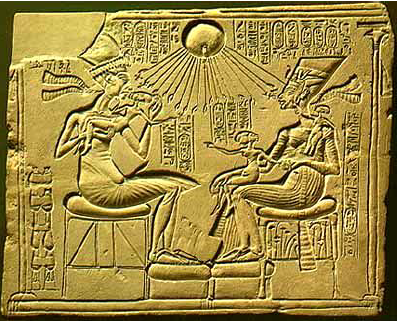
\includegraphics[width=1.0\linewidth]{01/ehnaton_nofertiti}}
\end{wrapfigure}

\paragraph{Echnaton Nofertitivel és gyermekeivel Aton istennek hódol}
Atont az égen középen lévő napkoronggal ábrázolták, amiből kezekben végződő sugarak áradnak szét. A dombormű a családot ábrázolja, amint a Atonhoz imádkozik. A már említett Amarna-kori stílusjegyek mellett megfigyelhetjük a figurák pókhasát, és a megnyúlt koponyákat.

\subsubsection*{Tutanhamon sírja}
Az egyiptomi régészet legnagyobb leletegyüttese egy mindössze 25 nm-es sírból származik: Tutankhamónéból. Ez volt az egyetlen olyan sír a XX.sz-ban, amit még nem raboltak ki a sírfosztogatók. Tutankhamón Echnaton után uralkodott, a Kr.e. XIV.sz. végén. Gyermekként, 8 éves korában koronázták meg, és helyette a papok vezették az országot, minthogy Echnaton halála után visszakerült a helyére az Amon-papság. Tutankhamón 19 éves koráig uralkodott, a történelem szempontjából nem volt jelentős fáraó, a sírjában talált 3 ezer darab tárgy, amit ma a kairói Egyiptomi Múzeum őriz, azonban az összes fáraó közül a leghíresebbé tette.

\paragraph{A feltárás története}
1922 novemberében egy brit régész, Howard Carter munkásai egy sima követ fedeztek fel egy másik sír mellett. Kiásták, és észrevették, hogy a kő egy lépcsőben folytatódik, majd egy 5 m mélyre vezető folyosóba torkoll. Carter akkor már 6 éve kereste Tutankhamon sírját, amiről tudni lehetett, hogy a Királyok völgyében van, de még senki nem találta meg. 


\begin{wrapfigure}{r}{0.35\textwidth}
	\tcbox[colback=darkgray!85!black,
	left=0mm,right=0mm,top=0mm,bottom=0mm,boxsep=1mm,toptitle=0.5mm,bottomtitle=0.5mm,
	title=\centering{Tutanhamon belső koporsójának másolata egy kiállításon}]{
		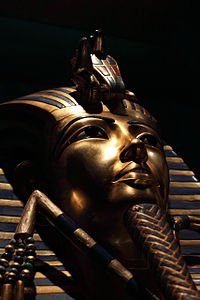
\includegraphics[width=1.0\linewidth]{01/tutanhamon_koporso}}
\end{wrapfigure}

Ennek az volt az oka, hogy míg a többi sír azonos szintben volt, addig Tutankhamón sírja egy másik alatt helyezkedett el. Carter ásatását egy szintén brit műkereskedő, Lord Carnarvon finanszírozta. Miután Carter eljutott az első befalazott ajtóig, értesítette Carnarvont, aki csak két hét múlva érekezett meg a helyszínre. Ekkor együtt bontották ki a falat, és a sír előszobájába érkeztek. A kis teremben nagy összevisszaságban számtalan tárgyat találtak: a fáraó harci szekereit, mindennapi eszközeit, aranyozott ágyakat, amiken mumifikálták, kisebb és nagyobb szobrokat, ékszereket, halotti áldozati ajándékokat. Azonnal nekiláttak a tárgyak katalogizálásához és elszállításához. Két héttel a sír felnyitása után azonban Lord Carnarvon ismeretlen okokból meghalt, amit a helyiek a fáraó átkaként értelmeztek. Elképzelhető, hogy a légmentes sírban mérgező gombák, baktériumok voltak, és ezek okozták Carnarvon halálát. Hamarosan az egyiptomi vezetők is észbe kaptak, és kitiltották Cartert a sírból, ám a brit kormánnyal való konfliktus elkerülése végett két év múlva visszaengedték. Csak ekkor tárta fel Carter a sírkamrát, ahol három egymásba helyezett két méter magas aranyozott fa-szentélyben (dobozban) megtalálta a fáraó vörös mészkő szarkofágját, ami szintén téglatest alakú volt. Ebben további három emberformájú szarkofágra lelt, kettő fából, és a legbelső színaranyból készült. Ebben feküdt Tutankhamón múmiája, amit később visszahelyeztek a sírba, máig is, nyugalomban, ott van. A múmia fején és mellkasán volt a lelet legjelntősebb tárgya: Tutankhamón aranymaszkja. Az aranyból készült halotti maszk az összeaszott arc eredeti, isteni harmóniáját kívánta feléleszteni: a fáraót idealizált portréban mutatja be. A szobron azonban reális törekvéseket is felfedezhetünk: a berakott szemek sarkaiban vörös festéknyomok fokozzák a valószerűséget. A nemesz-kendő csíkjai kék üvegpasztából készültek.

\paragraph{Tutanhamon halálának legendája}
Az 196o-as években megröntgenezték a fáraó koponyáját, és egy csontszilánkot találtak benne. Ekkor terjedt el az a vélemény, hogy a fáraót meggyilkolták, méghozzá fejbe vágták. A felnőtté vált Tutankhamón gyilkosságára utalt a sírban uralkodó rendetlenség is: valószínűnek tartották, hogy a fáraót gyorsan, titokban, sebtében temették el. A gyilkosság tényét erősítette meg az is, hogy a sírlelet-együttesben megtalálható egy különös tárgy, a fáraó arany lemezekkel díszített trónusa. A trónus azért érdekes, mert a háttámláján egy teljes mértékben Amarna-kori stílusjegyeket mutató dombormű található, amin Tutankhamón és felesége (a kartusról azonosítható, hogy őt ábrázolja a kép) elődjéhez hasonlóan Aton istenhez imádkozik. Ez arra utal, hogy felnőtt korában Tutankhamón is Aton-hívő volt, és az Amon-papságot, akik akkor már igen nagy befolyással bírtak, és kiskirályokként uralkodtak, meg akarta szüntetni. A fáraó halálának titokzatos körülményei máig izgatják a kutatókat: legutóbb 2oo5 februárjában vették ki a múmiát a sírból, és háromdimenziós digitális CT-vizsgálatnak vetették alá, ami azt az eredményt hozta, hogy talán még sem gyilkolták mega fáraót, hanem az egy baleset következtében súlyos térdsérülésben halt meg.

\clearpage

\section{Az ókor meghatározó festészeti techinkái: az egyiptomi falkép}

\begin{center}
	\begin{longtable}{ | m{0.25\textwidth} | p{0.75\textwidth} | }
		
		\hline
		\multicolumn{2}{|c|}{\textbf{A tétel adatai}}
		\\ \hline
		
		\hline
		Tétel teljes címe	
		 &
		 Melyek a meghatározó festészeti technikák az ókorban? Fejtse ki, miként alakult egy egyiptomi falkép elkészítésének munkamenete, milyen alapozást, pigmenteket és kötőanyagot használtak?
		\\ \hline
		
	\end{longtable}
\end{center}

\subsection*{Anyaghasználat az ókorban}

	Az ókor több szempontból is áttörést jelentett a festészet szemszögéből nézve. Az ember már ismeri a kötőanyagok fogalmát a festészetben, így olyan festékeket hoz létre, melyek tartós filmréteget képeznek, akár 2000 év elteltével is jó állapotban fennmaradtak, pl. Fayum múmia portrék, Pompeji faliképek stb. 

Kötőanyagnak elsősorban\textbf{ tojást, enyvet, viaszokat és néha növényi olajat} használtak.

Az ókori ember már tudott különböző, sokszor egészen bonyolult eljárásokkal létrehozni bizonyos színes pigmenteket, melyek addig nem álltak rendelkezésére. Pl. Ólomfehér, mínium, egyiptomi kék stb.

\subsection*{Festészeti technikák az ókorban}

\subsubsection{Egyiptom}

Egyiptom az ókori folyami kultúrák közé tartozó, gazdag és erős ország volt. A Nílus mentén
elterülő Alsó- és Felső-Egyiptom i.e. 2900-ban egyesült Ménész fáraó uralma alatt. Az ókori
Egyiptom történetét – ahogy a művészetét is korszakoljuk – három részre lehet osztani,
megkülönböztetve az uralkodókat, uralkodóházakat: az Óbirodalom (i.e. 2650-2150; III-VI.
dinasztia), a Középbirodalom (i.e. 2100-1750 körül, XI-XII. dinasztia), az Újbirodalom (i.e. 1550-
1070, XVIII-XX. dinasztia) kora. Egyiptom hanyatlani kezdett, i.e. IV. században Nagy
Sándor hódította meg.
Egyiptom nagyságához hozzájárult, hogy korán kialakult egy egységes írásrendszer, amely
elég fejlett volt nemcsak a mindennapi életben szükséges dolgok feljegyzéséhez, hanem a
tudományos felfedezések és az irodalmi alkotások leírásához is. Az egyiptomiak hite szerint a
halhatatlanságot az biztosította valaki számára, ha neve fennmaradt, ezért a legtöbben
igyekeztek legalább a nevüket feljegyeztetni a sírkamrákban.
Az egyiptomi írásrendszer megfejtése igen sokat segített az egyiptomi kultúra feltárásában, az
egyiptológia, mint tudományág kialakulásában. A hieroglifák bonyolult képírás, melyben
minden kis képnek külön jelentése van. A megfejtését a francia Jean-François Champollionnak köszönhetjük. 

\subsubsection{Az egyiptomi festészet}

Az élet mindennapi eseményeit örökítették meg, de általánosított, elvont formákkal. Az
alakok mérete változott, mégpedig aszerint, hogy milyen rangja volt életében.
A festmények a sziklasírokban, koporsókon fordultak elő. Jellemző rájuk, hogy az alakokat
szigorú szabályok szerint festették meg: nincs egységes nézőpont, több nézőpontból (oldal-,
elölnézet) ábrázolták ezeket. (legnagyobb felület törvénye). A síkszerű ábrázolás, szalagszerű
kompozíció, az egymás feletti elrendezést tiszta élénk színekkel emelték ki még jobban. 


\subsubsection{Ábrázolás az egyiptomi festészetben}

\paragraph{Kanonikus ábrázolás} \footnote{kanonikus jelentése: szabályos, törvényes, az egyházi törvényeknek megfelelő}
Az egyiptomi művészetben az alakok, tárgyak síkban való ábrázolására az Óbirodalom elején szigorú szabályok alakultak ki, amelyek végig megmaradtak. A művészek meghatározott mintákből dolgoztak. Az alakok megszerkesztéséhez négyzethálót alkalmaztak, ezáltal mind az alakok, mind a hireoglif jelek a rögzített arányrendszer szerint készültek. A művészeknek sok szabályt kellett megtartaniuk. Nem kívánták tőlük, hogy újat alkossanak, sőt, valószínűleg azt a művészt becsülték a legtöbbre, akinek munkái legjobban hasonlítottak a régi alkotásokhoz. Ebből a felfogásból adódott, hogy 3000 év alatt művészetük alig változott.

\paragraph{A művészet a halottkultusz szolgálatában}
A témákat megváltoztathatták, de az előadás módja, karaktere, lényegileg azonos maradt. Ennek alapján lehet ókori egyiptomi stílusról beszélni. Úgy képzelték, hogy a másvilágon a sírkamrákba helyezett szobrok dolgoznak az elhunyt helyett. A legtöbb alkotások sírokból kerültek elő: festmények a sírkamra falán, a halott szarkofágján, a halottakat a túlvilágon szolgáló szobrok és a neki odahelyezett edények, bútorok, a vele eltemetett ékszerek.

\paragraph{Jellemzői} Nincs árnyékolás, különböző nézőponti ábrázolás, állatok ábrázolása, térbeliség ábrázolása, stilizálás, díszítés, nem a látszat szerint festettek hanem a törvények alapján, templomok festése, egymás utáni szituációk ábrázolása.


\subsubsection{Az egyiptomi festészet jellemzői}
\begin{compactitem}
	\item Érvényesül a \textbf{legnagyobb felület törvénye}: az arc,  kar, a láb oldalnézetben van, a szem, a váll, a mellkas és törzs pedig elölnézetben, csípő 3/4 profilban.
	\item Kanonizált és jelképes (a fej mindig profilban van, a szem szemből, a törzs deréktól
	fölfelé elölnézetben, a mell oldalról, a test csípőtől lefelé szintén oldalról látszik stb.)
	\item A jeleneteket síkban kiterítik.
	\item Képregényszerű jelenetek.
	\item Az egymás mögöttiséget egymás fölöttiséggel helyettesítik.
	\item A mozgás mindig arra tart amerre mutatnak a képcsíkok.
	\item Nincs egyetlen nézőpont és térbeli mélység.
	\item A színek tiszták, élénkek. Használják a barnát, okkert, sárgát, kéket, zöldet, pirosat,
	feketét, fehéret.
	\item A képeknek van ritmusuk.
	\item Az alakok részben takarhatják egymást.
	\item Eszköz: földfesték, nádecset.
\end{compactitem}

\begin{figure}[H]
	\centering
	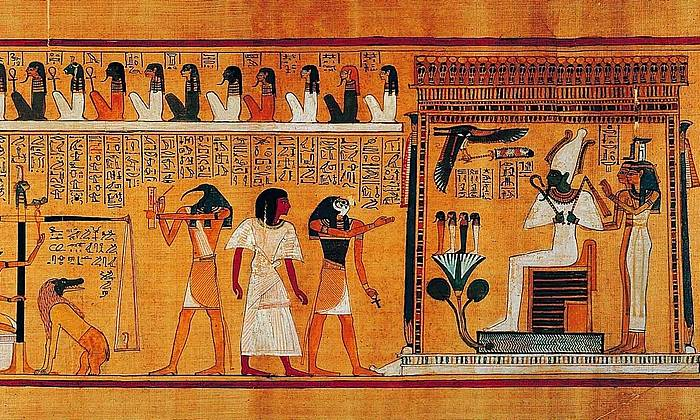
\includegraphics[width=0.8\linewidth]{01/egyiptom}
\end{figure}


\subsubsection*{Az ókori görög festészet jellemzői}

\begin{compactitem}
	\item Növény- és állatmotívumos díszítés a leggyakoribb.
	\item A megmaradt emlékek közül a legjelentősebb alkotások a festett vázák.
	\item A vázaképke a görög élet és mitológia érdekes jeleneteit mutatják be.
	\item Archaikus kor: feketealakos vázafestés (eredeti/fehér csempeszín + fekete vázafestés).
	\item Klasszikus kor: vörösalakos vázafestés (fekete háttér + vörösre festett alakok).
\end{compactitem}


\subsection*{Az egyiptomi falkép elkészítésének munkamenete}

Az egyiptomi vakolatok fő anyaga a nílusi iszap: agyag, homok, mész és gipsz keveréke. A kötőanyag kérdése eldöntetlen, lehet gipsz is, mész is.

\begin{itemize}
	\item \textbf{A fal előkészítése:} 
	\begin{compactitem}
		\item Sima kőfelület esetén: vékony gipsz vakolat.
		\item Durva felület esetén: agyagos, vastagabb simító vakolat, erre vékony gipszes vakolás. Ilyen felületeken az esetleges domborítás a vakolatból készült.
	\end{compactitem}
	
	\item \textbf{Festék:} tempera.
	
	\item \textbf{Pigmentek:} okkerek, korom, mész, egyiptomi kék és zöld.
	
	\item \textbf{Előrajz:} fonalpattintással jelölték ki a főbb tengelyeket
	valamint a szinteket, és alakították ki a figurák arányait megadó hálózatot. A kompozíciót vörös festékkel rajzolták fel, és feketével korrigálták.
	
	\item \textbf{Festés:} először az alapszíneket festették fel síkszerűen és
	fedő módon. Az előrajzok ettől teljesen eltűntek. Ezután az egyre finomabb részletek, majd pedig a végső kontúrok következtek.
	
	\item \textbf{Lakkozás:} a sárga és vörös felületeken a 18. dinasztia idejében gyakran előfordul, a sárgák esetében talán az arany-
	hatás imitálására. A Nefertari sír sárga és vörös felületein gyantát és tojásfehérjét találtak a lakkozott felületeken, de korukat nem tudták megállapítani. Lehettek esetleg későbbi fixálások eredményei is.
\end{itemize}

\section{Galéria}

\begin{figure}[H]
	\begin{minipage}{0.4\textwidth}
		\tcbox[colback=darkgray!85!black,
		left=0mm,right=0mm,top=0mm,bottom=0mm,boxsep=1mm,toptitle=0.5mm,bottomtitle=0.5mm,
		title=\centering{Dzsószer fáraó lépcsős piramisa}]{
			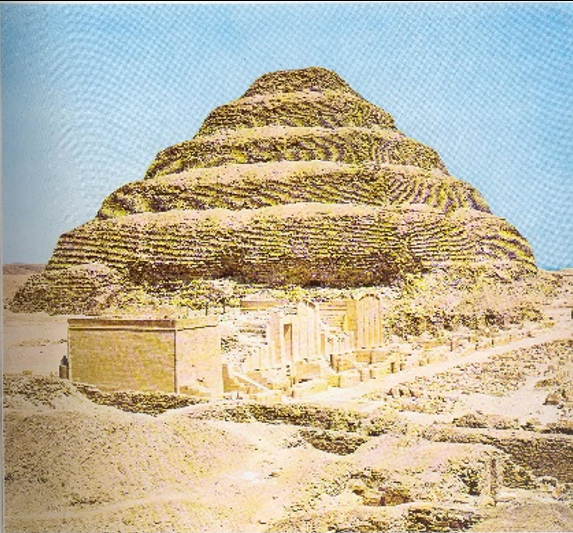
\includegraphics[width=1.0\linewidth]{01/04_lepcsos_piramis}}
	\end{minipage}
	\hfill
	\begin{minipage}{0.55\textwidth}
		\tcbox[colback=darkgray!85!black,
		left=0mm,right=0mm,top=0mm,bottom=0mm,boxsep=1mm,toptitle=0.5mm,bottomtitle=0.5mm,
		title=\centering{Piramis keresztmetszet}]{
				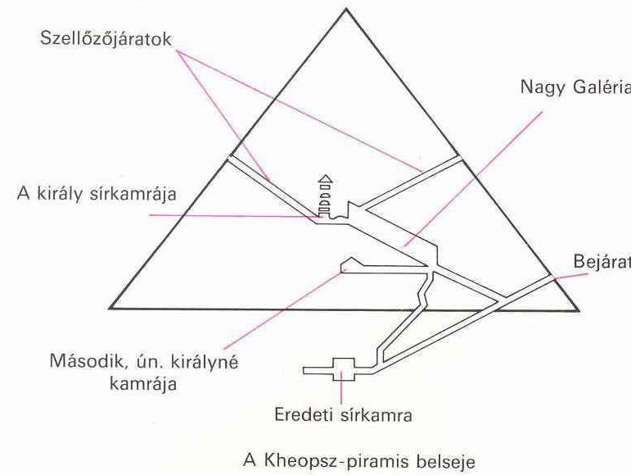
\includegraphics[width=1.0\linewidth]{01/02_piramis_keresztmetszet}}
	\end{minipage}

	\begin{minipage}{0.47\textwidth}
		\tcbox[colback=darkgray!85!black,
		left=0mm,right=0mm,top=0mm,bottom=0mm,boxsep=1mm,toptitle=0.5mm,bottomtitle=0.5mm,
		title=\centering{Masztaba}]{
			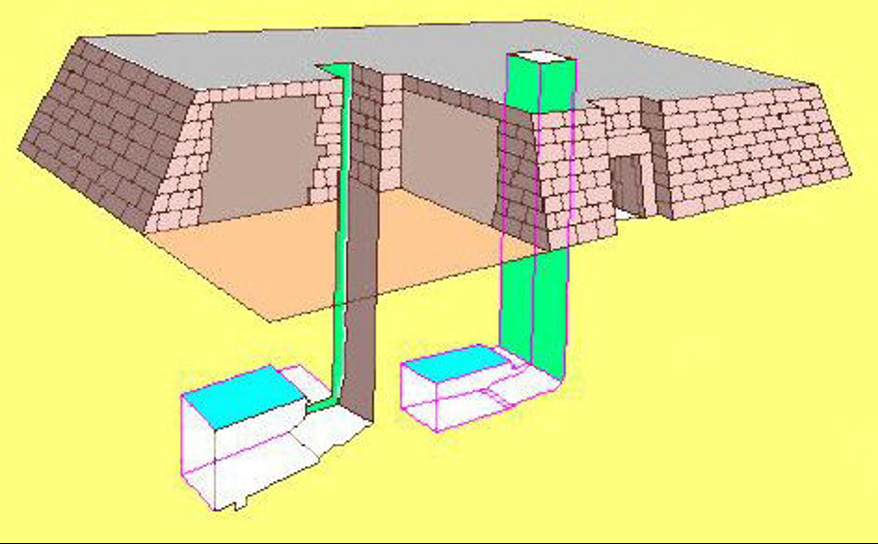
\includegraphics[width=1.0\linewidth]{01/03_masztaba}}
	\end{minipage}
	\hfill
	\begin{minipage}{0.47\textwidth}
		\tcbox[colback=darkgray!85!black,
		left=0mm,right=0mm,top=0mm,bottom=0mm,boxsep=1mm,toptitle=0.5mm,bottomtitle=0.5mm,
		title=\centering{Gízai piramisok}]{
			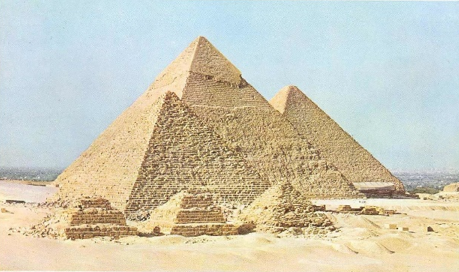
\includegraphics[width=1.0\linewidth]{01/01_gizai_piramisok}}
	\end{minipage}
\end{figure}

\begin{figure}[H]
	\begin{minipage}{0.35\textwidth}
		\tcbox[colback=darkgray!85!black,
		left=0mm,right=0mm,top=0mm,bottom=0mm,boxsep=1mm,toptitle=0.5mm,bottomtitle=0.5mm,
		title=\centering{Sziklasír}]{
			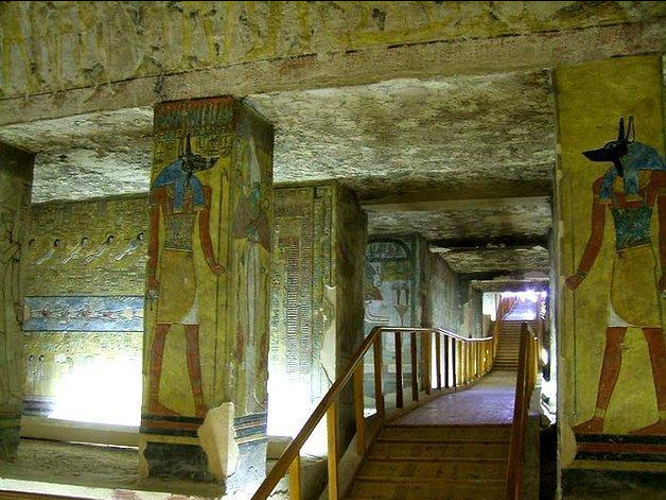
\includegraphics[width=1.0\linewidth]{01/05_sziklasir}}
	\end{minipage}
	\hfill
	\begin{minipage}{0.6\textwidth}
		\tcbox[colback=darkgray!85!black,
		left=0mm,right=0mm,top=0mm,bottom=0mm,boxsep=1mm,toptitle=0.5mm,bottomtitle=0.5mm,
		title=\centering{Luxori templom alaprajza}]{
			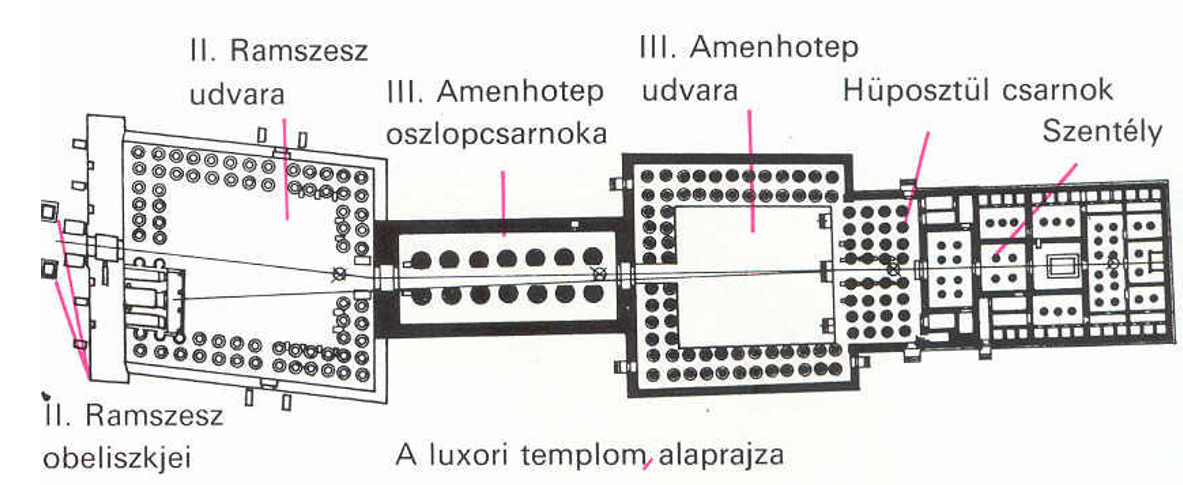
\includegraphics[width=1.0\linewidth]{01/06_luxori_templom}}
	\end{minipage}
	
	\begin{minipage}{0.43\textwidth}
		\tcbox[colback=darkgray!85!black,
		left=0mm,right=0mm,top=0mm,bottom=0mm,boxsep=1mm,toptitle=0.5mm,bottomtitle=0.5mm,
		title=\centering{Karnaki templom}]{
			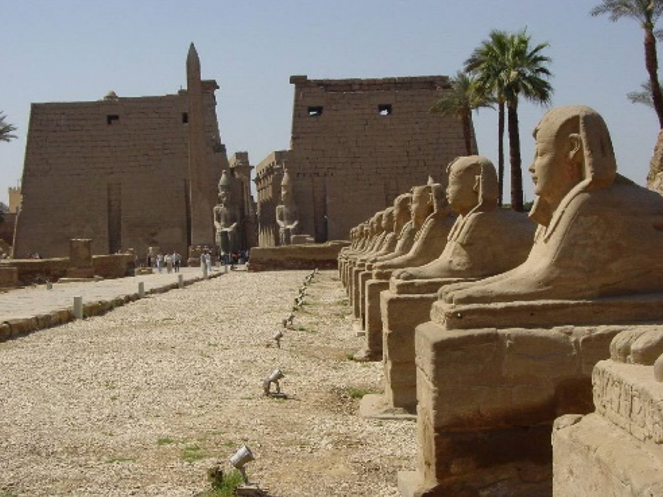
\includegraphics[width=1.0\linewidth]{01/07_karnak}}
	\end{minipage}
	\hfill
	\begin{minipage}{0.43\textwidth}
		\tcbox[colback=darkgray!85!black,
		left=0mm,right=0mm,top=0mm,bottom=0mm,boxsep=1mm,toptitle=0.5mm,bottomtitle=0.5mm,
		title=\centering{Karnaki templom udvara}]{
			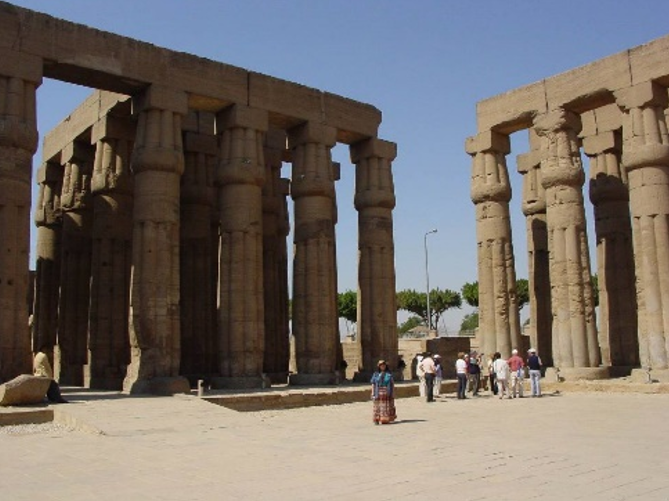
\includegraphics[width=1.0\linewidth]{01/08_karnak}}
	\end{minipage}

	\begin{minipage}{0.15\textwidth}
		\tcbox[colback=darkgray!85!black,
		left=0mm,right=0mm,top=0mm,bottom=0mm,boxsep=1mm,toptitle=0.5mm,bottomtitle=0.5mm,
		title=\centering{Legnagyobb felületek törvénye}]{
			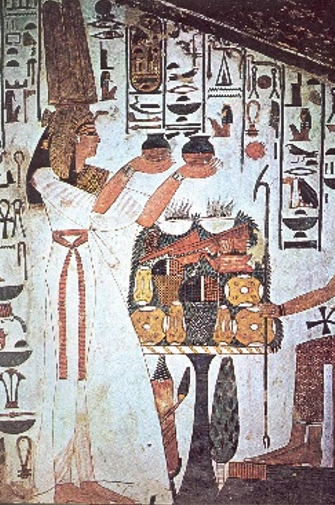
\includegraphics[width=1.0\linewidth]{01/09_feluletek}}
	\end{minipage}
	\hfill
	\begin{minipage}{0.4\textwidth}
		\tcbox[colback=darkgray!85!black,
		left=0mm,right=0mm,top=0mm,bottom=0mm,boxsep=1mm,toptitle=0.5mm,bottomtitle=0.5mm,
		title=\centering{Gízai szfinx}]{
			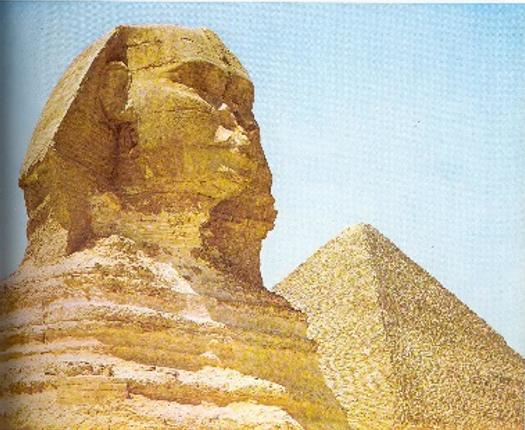
\includegraphics[width=1.0\linewidth]{01/10_gizai_szfinx}}
	\end{minipage}
	\hfill
	\begin{minipage}{0.2\textwidth}
		\tcbox[colback=darkgray!85!black,
		left=0mm,right=0mm,top=0mm,bottom=0mm,boxsep=1mm,toptitle=0.5mm,bottomtitle=0.5mm,
		title=\centering{Tutanhamon aranymaszkja}]{
			\includegraphics[width=1.0\linewidth]{01/11_tutanhamon}}
	\end{minipage}

	\begin{minipage}{0.25\textwidth}
		\tcbox[colback=darkgray!85!black,
		left=0mm,right=0mm,top=0mm,bottom=0mm,boxsep=1mm,toptitle=0.5mm,bottomtitle=0.5mm,
		title=\centering{Kefrén szobra}]{
			\includegraphics[width=1.0\linewidth]{01/12_kefren}}
	\end{minipage}
	\hfill
	\begin{minipage}{0.35\textwidth}
		\tcbox[colback=darkgray!85!black,
		left=0mm,right=0mm,top=0mm,bottom=0mm,boxsep=1mm,toptitle=0.5mm,bottomtitle=0.5mm,
		title=\centering{Nofertiti büsztje}]{
			\includegraphics[width=1.0\linewidth]{01/nofertiti}}
	\end{minipage}
	\hfill
	\begin{minipage}{0.16\textwidth}
		\tcbox[colback=darkgray!85!black,
		left=0mm,right=0mm,top=0mm,bottom=0mm,boxsep=1mm,toptitle=0.5mm,bottomtitle=0.5mm,
		title=\centering{Ehnaton szobra}]{
			\includegraphics[width=1.0\linewidth]{01/ehnaton}}
	\end{minipage}

\end{figure}

\cleardoublepage

\chapter{Az antik görög művészet}
\label{ch:2_antik_gorog}

\section{Az antik görög kor hitvilága, korszakai és építészete}

\begin{center}
	\begin{longtable}{ | p{0.2\textwidth} | p{0.8\textwidth} | }
		
		\hline
		\multicolumn{2}{|c|}{\textbf{A tétel adatai}}
		\\ \hline
		
		\hline
		Tétel teljes címe & Mutassa be az antik görög kor hitvilágát, korszakait és építészetét! Elemezze a legismertebb épületeit, művészeti alkotásait!
		\\ \hline
		
		Jegyzetek &
		\begin{compactitem}
			\item Az ókori görög művészet és kultúra korszakai, jellemzői.
			\item A templomok felépítése, az oszloprendek jellemzői.
			\item A görög szobrászat jellegzetes vonásai a különböző korszakokban.
			\item A görög mitológia világa, a görög vázafestészet.
		\end{compactitem}
		\\\hline
		
	\end{longtable}
\end{center}

\cleardoublepage

\section{Az ókori görög kultúra festészetének hatása a római kori festészetre}

\begin{center}
	\begin{longtable}{ | p{0.2\textwidth} | p{0.8\textwidth} | }
		
		\hline
		\multicolumn{2}{|c|}{\textbf{A tétel adatai}}
		\\ \hline
		
		\hline
		Tétel teljes címe &
		Milyen módon, mértékben hatottak az ókori görög kultúra festészeti megoldásai tartalmi, formai, technikai szempontból a római kor festészetére? Milyen ókori mozaiktechnikákat ismer?
		\\ \hline
		
	\end{longtable}
\end{center}

\cleardoublepage

\chapter{Az antik Róma művészete} % Introduction
\label{ch:3_antik_roma}

\section{Az antik Róma korszakai, kultúrája, építészete, szobrászata és festészete}

\begin{center}
	\begin{longtable}{ | p{0.2\textwidth} | p{0.8\textwidth} | }
		
		\hline
		\multicolumn{2}{|c|}{\textbf{A tétel adatai}}
		\\ \hline
		
		\hline
		Tétel teljes címe & 
		\\ \hline
		
		Jegyzetek &
		\begin{compactitem}
			\item Jegyzet
		\end{compactitem}
		\\\hline
		
	\end{longtable}
\end{center}


\section{A római kori festészet alapvető jellemzői}

\begin{center}
	\begin{longtable}{ | p{0.2\textwidth} | p{0.8\textwidth} | }
		
		\hline
		\multicolumn{2}{|c|}{\textbf{A tétel adatai}}
		\\ \hline
		
		\hline
		Tétel teljes címe 
		&
		
		\\ \hline
		
	\end{longtable}
\end{center}
\cleardoublepage

\chapter{Minta tétel} % Introduction
\label{ch:minta}

\section{Egy egy minta cím}

\paragraph{Egy egy minta paragrafus}

\lipsum[1-2]

\cleardoublepage

\chapter{A románkori művészet} % Introduction
\label{ch:5_romankor}

\section{A románkori építészet, szobrászat és kézművesség}


\tcbox[left=0mm,right=0mm,top=0mm,bottom=0mm,boxsep=0mm,
toptitle=0.5mm,bottomtitle=0.5mm,title=\centering{A tétel adatai}]{%
	
	\begin{tabular}{| p{0.25\textwidth} | p{0.7\textwidth} |}

		\hline
		\centering{Tétel teljes címe}
		&
		Mutassa be a románkori építészet, szobrászat és kézművesség stílusjegyeit! Jellemezze a különböző műfajokhoz kapcsolódó alkotásokat, európai és hazai műemlékeinket!
		\\ \hline
		
		\centering{Jegyzetek}
		&
		\begin{compactitem}
			\item A románkor társadalma, hitvilága, építészete.
			\item A koraközépkori szobrászat, kódexfestészet és kézművesség jellemzői.
		\end{compactitem}
		\\\hline
		
	\end{tabular}}

	\subsection*{Bevezetés}
	
		\paragraph{Földrajzi elhelyezése}
		A román kor a népvándorlás kora után kialakuló nyugat-európai (elsősorban a német, francia nyelvterületek és itáliai), kereszténységet fölvett államok művészete.
		Az első keresztény állam létrejöttétől (Frank Birodalom Nagy Károly vezetésével kb. 800-tól) a IX., X., XI. századon át a XII. század végéig, a gótika elterjedéséig számítjuk.
		
		\paragraph{Korszakai}
		A IX., X. századot korai román, vagy preromán („pre” = valami előtti) kornak nevezzük.
		A XI., XII. század a korszak virágkora, ezért ezt érett román kornak nevezzük.
		
		\paragraph{Kifejezés eredete, jelentése}
		A kifejezés 19. századi eredetű. A nyugati nyelvekből került magyar nyelvbe, a nyugati szakkifejezés hangalakjának átvételével. A magyar kifejezésnek azonban semmi köze a román nyelvhez és népcsoporthoz, annál több az antik római kor építészetéhez. A román kori építészetben az ókori Róma építészetének hatását, vonásait fedezhetjük fel – a kifejezés jelentése tehát nem „román”, hanem római.
	
		\paragraph{Római hatások}
		\begin{compactitem}
			\item A román kor építészete az antik római építészet hatását mutatja: azzal kapcsolódik a római építészethez leginkább, hogy nyílásai, boltozatai félkörívesek. (A 19. században „félköríves stílnek” is nevezték megkülönböztetve az utána következő gótikától, ami a „csúcsíves stíl” nevet viselte).
			
			\item A román kor művészete abban „római”, „rómaias” még, hogy a vele egy időben virágkorát élő Bizánc művészetével szemben nem a keleti, ortodox, hanem a nyugati, Róma-központú keresztény egyház művészete.
			
			\item További „római” vonás a korban, hogy a korai román kor uralkodói – Nagy Károly, Ottók – arra törekedtek, hogy államaikkal az egykori antik nyugat-római birodalmat élesszék fel egyfajta „keresztény római birodalom” formájában.
		\end{compactitem}
	
	\subsection*{Kultúrtörténeti háttér}
		
		A román kor az Európába vándorolt „barbár” népek letelepülésével, államalapításával, a kereszténység felvételével kezdődik. A legjelentősebb ilyen megszilárdult keresztény állam a Frank Birodalom. A Frank Birodalom uralkodója Nagy károly, aki a római pápával 800-ban császárrá koronáztatja magát. Császársága az egykori nyugat-római birodalom jogutódja kíván lenni, és a Keleten virágzó Bizánc nyugati riválisa is, ezért fél évszázadnyi időre Nagy Károly Európa nagy részét fennhatósága alá vonja.
		
		\paragraph{A Német-Római Birodalom kialakulása}
		a X. században a német területek erősödnek meg: a német Ottó nevű uralkodók veszik át az irányítást. A frank állam hanyatlása, majd a kalandozó magyarok legyőzése után I. Ottó koronáztatja magát császárrá Rómában, és létrehozza a Német-Római Birodalmat szintén az egykori antik Róma felélesztésének szándékával. A Nyugat-Római Birodalom a XI-XII. században is Európa legnagyobb hatalommal bíró állama marad.
		
		\paragraph{A pápai állam vagy egyházi állam}
		A román kor alatt még egy jelentős állam jön létre: az Egyházi állam Közép-Itália területén. Ezzel a nyugati egyház politikai hatalomra is szert tesz Európában, és a művészetek legfőbb megrendelőjévé válik: templomokat épített, azok szobrászi és festészeti díszítését irányítja. Így a román kor művészete nagy részt szakrális, azaz vallásos célú. Tovább fokozza az egyház hatalmát Nyugat- és Közép-Európa területén az ún. egyházszakadás: 1054-ben az addig egységes keresztény egyház ketté válik: nyugati-római egyházzá és keleti, ortodox egyházzá.
		
		\paragraph{Szerzetesrendek}
		A román korban igen nagy szerepet töltenek be a népvándorlás alatt megszülető szerzetesrendek, melyek a betelepülő „barbár”népek megtérítésének, majd az új keresztény államokban a keresztény vallás terjesztésének érdekében jönnek létre. A terjesztésben a művészetet hívják segítségül: a templom-építészetben, kolostor-építészetben, a templomok, kolostorok szobrászati díszítésében, a kódexfestészetben jeleskednek. A leghíresebb román kori szerzetesrend a bencés rend (Szent Benedek alapítja).
		
		\paragraph{Keresztes hadjáratok}
		A román kor idején az egyház keresztes hadjáratokat indít, melyek a pápa által szentesített, a keresztes lovagok részvételével folytatott nagyarányú hadjáratok voltak a 11–13. században. Fő céljuk a Szentföld megszerzése volt a muszlim araboktól és törököktől, de a spanyol nyelvterületen előrenyomuló mórok (spanyolországi arabok, afrikaiak) ellen is.
		
		
	\subsection*{Templomépítészet}
	
	Ebben a koprszakban templomok, kolostorok és várak épülnek leginkább.
	
	\subsubsection{Külső jellemzők}
	
	A templom az egyház megerősödő hatalmát, az egyház által nyújtott védelmet van hívatva kifejezni, ezért külseje biztonságot, erőt, megingathatatlanságot sugall.
	\begin{compactitem}
		\item A külső zárt, csak kisméretű nyílásokkal van áttörve.
		\item A tömegek zárt, egyszerű, tömbszerű, gyakran egészen a geometriai.
		formákig leegyszerűsített hasáb-, henger- és kockaszerű egységek.
		\item A templomot vaskos, masszív, robosztus tömegek alkotják.
		\item A külső puritán, azaz alig díszített.
	\end{compactitem}

	\subsubsection{Alaprajz}
	
	A templom alaprajza a keresztény egyház szertartásainak rendje szerint alakul: követi az ókeresztény bazilikák formáját.
	\begin{compactitem}
		\item Hosszanti elrendezésű,
		\item három vagy öt hajós,
		\item keletelt: azaz keleti oldalán helyezkedik el a félkörívű apszis, a szentély,
		\item az apszis előtt négyezeti tér és kereszthajó található.
	\end{compactitem}

	\subsubsection{Szerkezet}
	
	\begin{wrapfigure}{r}{0.2\textwidth}
		\tcbox[colback=darkgray!85!black,
		left=0mm,right=0mm,top=0mm,bottom=0mm,boxsep=1mm,toptitle=0.5mm,bottomtitle=0.5mm,
		title=\centering{Kockafejezet}]{
			\includegraphics[width=1.0\linewidth]{05/kockafejezet}
		}
	\end{wrapfigure}
	
	A templomok bazilikális szerkezetűek, azaz
	főhajójuk kiemelkedik a mellékhajók fölött, és a belső
	tér a kiemelkedő falakon nyitott ablakokon keresztül
	kapja a megvilágítást.
	
	Az ablakok kis méretűek, a falak tehát kevéssé vannak áttörve, vastagok,
	masszívak, erősek, további külső megtámasztás nélkül viselik a boltozat súlyát.
	
	A román templomok belső súlyt hordó tartóelemei
	egyszerű, hasábszerű pillérek, vagy tömzsi oszlopok. Az oszlopfejezetek gyakran minden díszítést nélkülöző, kocka formájú oszlopfők – ezek az ún. „\textbf{kockafejezetek}”.
	
	\subsubsection{Külső díszítőelemek}
	
	A templomok kevéssé díszítettek, de a falfelületeket nyílások, függőleges és vízszintes elemek tagolják.
	
	\paragraph{Bélletes kapuzat}
	A román kori templomok legjellemzőbb homlokzati
	eleme, a befelé szűkülő, a kapu körül ívben végigfutó féloszlopokkal díszített
	félköríves kapuzat. A bélletek (a kapu fölött futó féloszlopok) gyakran
	geomertikus mintákkal, fogsor-motívummal, cikk-cakk mintával faragott.
	
	\paragraph{Lőrészszerű ablak}
	Kis ablaktípus, keskeny, felül íves, befelé szűkül.
	
	\paragraph{Ikerablak}
	Kettős vagy hármas ablak, felül ívesek (félkör) az ablakok
	között kis oszlopok vannak.
	
	\paragraph{Ívsor vagy ívpárkányzat}
	Vízszintes tagolóelem, ami a külsőn jelzi a belső
	szinteket: kis ívek sorakoznak egymás mellett.
	
	\paragraph{Törpegaléria}
	Apró árkádok (kis boltívek és kis oszlopok), árkád a homlokzaton, ami mögött egy keskeny fal húzódik.
	
	\paragraph{Vakárkád}
	A homlokzaton ált. alul található olyan árkádok ami alatt, nem lehet
	átmenni, mert be vannak falazva tehát csak díszítő szerepük van.
	
	\paragraph{Féloszlop}
	A falhoz tapadó, függőlegesen félbevágott oszlop (oszlop-lábazata,
	oszlopfője van).
	
	\paragraph{Pilaszter}
	A falból négyzetesen kiugró (oszlopszerű) falsáv, amelynek fejezete és
	lábazata van.
	
	\paragraph{Lizéna}
	A falból négyzetesen kiugró falsáv fejezet és lábazat nélkül.
	
	
	\subsubsection{Térlefedés}
	
	A templomok boltozási rendszere az antik Róma idején kialakult boltozást: a donga és keresztboltozatot fejleszti tovább.
	
	A leggyakoribb boltozattípus a „román
	keresztboltozat” = két félhenger alakú dongaboltozat
	kereszteződése négyzet alaprajzon.
	
	A román keresztboltozatnak két típusa alakult ki.
	
	\paragraph{Élkeresztboltozat}
	Az íves falrészek megerősítés nélkül élekben találkoznak.
	
	\paragraph{Bordás keresztboltozat}
	az íves falrészek találkozásánál a boltozatot bordákkal erősítik meg, a bordák, amiket erős, súlyosabb kövekből raknak ki levezetik a boltozat súlyát az oldalfalakra, így a köztük lévő falakat könnyebb kövekből lehet rakni (Ez a típus alakul ki időben később, a XII. sz.-ban).
	
	\paragraph{Kötött térrendszer}
	A boltozás rendszere, logikája: ún. „kötött térrendszer” v. ,,kötött boltozás”. Mivel csak négyzet alaprajzú tereket tudtak lefedni, kialakult az a rendszer, hogy a főhajó egy boltszakaszára a mellékhajóban két fele akkora négyzetes boltszakasz kerül: hevederívek, a boltszakaszokat egymástól elválasztó ívek.
	
	\begin{figure}[H]
		\centering
		\begin{minipage}{0.45\textwidth}
			\tcbox[colback=darkgray!85!black,
			left=0mm,right=0mm,top=0mm,bottom=0mm,boxsep=1mm,toptitle=0.5mm,bottomtitle=0.5mm,
			title=\centering{Keresztboltozat}]{
				\includegraphics[width=1.0\linewidth]{05/keresztboltozat}
			}
		\end{minipage}
		\hfill
		\begin{minipage}{0.5\textwidth}
			
			\tcbox[colback=darkgray!85!black,
			left=0mm,right=0mm,top=0mm,bottom=0mm,boxsep=1mm,toptitle=0.5mm,bottomtitle=0.5mm,
			title=\centering{Kötött térrendszer}]{
				\includegraphics[width=1.0\linewidth]{05/kotott_terrendszer}
			}
		\end{minipage}
	\end{figure}

	\subsubsection{Német építészet}
	
	A német román templomok leghíresebb példái:
	a Német- Római császárok által épített dómok, ún. ,, császárdómok”: Hildesheim-i Szent Mihály templom, Maria Laach dómja, Speyer-i császárdóm, Worms-i császári dóm.
	
	\begin{figure}[H]
		\centering
		\begin{minipage}{0.3\textwidth}
			\tcbox[colback=darkgray!85!black,
			left=0mm,right=0mm,top=0mm,bottom=0mm,boxsep=1mm,toptitle=0.5mm,bottomtitle=0.5mm,
			title=\centering{Hildesheim-i Szent Mihály templom}]{
				\includegraphics[width=1.0\linewidth]{05/hildesheim.jpg}
			}
		\end{minipage}
		\hfill
		\begin{minipage}{0.3\textwidth}
			
			\tcbox[colback=darkgray!85!black,
			left=0mm,right=0mm,top=0mm,bottom=0mm,boxsep=1mm,toptitle=0.5mm,bottomtitle=0.5mm,
			title=\centering{Maria Laach dóm}]{
				\includegraphics[width=1.0\linewidth]{05/maria_laach}
			}
		\end{minipage}
	\hfill
	\begin{minipage}{0.34\textwidth}
	
		\tcbox[colback=darkgray!85!black,
		left=0mm,right=0mm,top=0mm,bottom=0mm,boxsep=1mm,toptitle=0.5mm,bottomtitle=0.5mm,
		title=\centering{Speyer-i császárdóm}]{
			\includegraphics[width=1.0\linewidth]{05/speyer}
		}
	\end{minipage}
	\end{figure}
	
	
	\subsubsection{Itáliai építészet}
	
	\paragraph{Sajátosságai}
	Az itáliai építészet sajátosságai, hogy
	\begin{compactitem}
		\item a templomok három épületegységből állnak
		\item gyakori a márványburkolat
		\item gyakori az ún. „oroszlános kapuzat”
	\end{compactitem}

	\paragraph{Épületei}
	A templomhoz, azaz a dómhoz további két, külön álló épület kapcsolódik. A campanile, azaz harangtorony és a baptisztérium, azaz keresztelő kápolna. A kifejezés a latin baptistero (jelentése keresztelés) szóból ered. A
	baptisztérium olyan épület, ami a templom nyugati
	homlokzatával szemben áll, centrális alaprajzú, és benne
	egy szintén centrális keresztelő medence található a
	keresztelés szertartásának végzésére.
	
	A három részes román épületegyüttesek leghíresebb példája:
	a Pisa-i épületegyüttes.
	
	\paragraph{Pisai dóm}
	
	\subparagraph{Alaprajz}
	Alaprajza olyan mintha 3 bazilikából állna: 5-hajós hosszház + 2 háromhajós
	keresztház.
	
	\subparagraph{Külső tömeg}
	Hangsúlyos négyzeti tér alakul ki, ami fölött az itáliai
	építészetben a német templomok szögletes, sátortetős négyzeti tornyaitól
	eltérően íves, kupolához hasonló térlefedés van.
	
	\subparagraph{Homokzat}
	Legfőbb homlokzati díszek a törpegalériák (4 szinten), alul
	vakárkádok. A homlokzat teljes felületét márványburkolat díszíti
	
	\subparagraph{Belső tér} Márvány burkolat (csíkos), nyitott fa fedélszék
	
	\subparagraph{Szerkezet} Jól láthatóan bazilikás.
	
	\subparagraph{Pisai keresztelőkápolna (baptistérium)}
	Alaprajza kör alakú.
	
	Külseje követi a dóm díszítését - vakárkádos, törpegalériás ez is
	(a felső szintek már a gótika jegyében készültek, ezért felül fiatornyok, növényi faragványok is láthatók).
	
	
	
	\begin{wrapfigure}{r}{0.45\textwidth}
		\tcbox[colback=darkgray!85!black,
		left=0mm,right=0mm,top=0mm,bottom=0mm,boxsep=1mm,toptitle=0.5mm,bottomtitle=0.5mm,
		title=\centering{Pisa-i épületegyüttes}]{
			\includegraphics[width=1.0\linewidth]{05/pisa}
		}
	\end{wrapfigure}
	
	\subparagraph{Pisai "ferdetorony" (campanile)}
	Illeszkedik a dóm és a baptisztérium külső díszítéséhez: alul itt is vakárkádok, a felső szinteken törpegalériák találhatók; legfelül félköríves nyílások között a harangok; kör alaprajzú
		
	Már építése közben is elkezdett süllyedni, a 3 szint után megváltoztatták a dőlésszöget, hogy ne ferdüljön tovább, de már késő volt, az épület tovább süllyedt.
	
	\paragraph{Márványinkrusztáció}
	Az itáliai templomok különösen Firenzében elterjedt, gyakori díszítési módja a márványinkrusztáció, azaz színes márványlapokból kialakított burkolat. A márványlapok gyakran geometrikus mintát mutatnak, vagy faltagoló elemeket, pl. törpegalériát, ablakot, kapunyílást imitálnak.
	
	\paragraph{Oroszlános kapuzat}
	Észak-Itália templomainak leggyakoribb jellemzője az „oroszlános kapuzat”
	Az egyébként viszonylag díszítetlen templomhomlokzaton a kapu fölött baldachin található, aminek súlyát egy-egy oroszlánra támaszkodó oszlop tartja. A kaput őrző oroszlán motívuma a művészettörténetben a védelem szimbóluma.
	
	\subsubsection{A Cluny bencés apátság}
	
	\begin{wrapfigure}{r}{0.45\textwidth}
		\tcbox[colback=darkgray!85!black,
		left=0mm,right=0mm,top=0mm,bottom=0mm,boxsep=1mm,toptitle=0.5mm,bottomtitle=0.5mm,
		title=\centering{A Cluny bencés apátság makettje}]{
			\includegraphics[width=1.0\linewidth]{05/cluny}
		}
	\end{wrapfigure}
	
	A román kori szerzetesi építészet jelentőségét, magas művészi értékét, gazdagságát a leghíresebb román kori szerzetesrend, a bencések \textbf{franciaország}i, Cluny-ben található kolostora példázza. A hatalmas épületegyüttesből mára mindössze a nagyobbik kereszthajó déli szárnya maradt meg, a többi rész robbantások áldozata lett. Az egykori impozáns épületegyüttesről rekonstrukciós rajzok és makettek alapján tájékozódhatunk.
	
	A bencés apátságok önálló, saját gazdasággal rendelkező kisvárosok voltak. Természetesen központjukban mindig a templom állt, amellett volt található a kolostor épülete.
	
	\paragraph{Kolostor-templom}
	Hatalmas méretű, monumentális épület volt: hosszháza 5 hajóból állt, amihez 3 hajós (!) előcsarnok csatlakozott, továbbá a templomnak 2 keresztháza volt. Az alaprajz tehát bonyolult volt, nagyon gazdag, számos kis épületrészből állt.
	
	\paragraph{A kolostor részei}
	A templomokhoz kapcsolódó kolostorok mindig azonos rend, alaprajz szerint épültek fel.
		
		\subparagraph{Kerengő}
		Azz ókeresztény átrium teréből kialakuló, elmélkedésre szolgáló, négyzet alaprajzú, árkádos folyóval körbevett udvar volt a központ.
		
		\subparagraph{Reflektórium}
		A kerenmgőből nyíló szerzetesi ebédlő, ált. egy hosszúkás terem.
		
		\subparagraph{Dormitórium}
		Szintén a kerengőből nyíló, szerzetesi alvóhely.
		
	A kolostorhoz konyha, temető, kórház, gazdasági egységek, vendégház, istálló, kert, veteményes, pékség, és további, az önálló szerzetesi élethez szükséges épületek csatlakoztak.
	
	\subsection*{Szobrászat}
	
		A szobrászati alkotások az épületekhez kapcsolódnak, domborművek (csak ritka esetben szabadon álló körplasztikák).
		\begin{compactitem}
			\item Az épület nyugati homlokzatán található domborművek.
			\item A kapu fölötti íves timpanonban lévő domborművek.
			\item Figurális oszlopfejezetek az épületbelsőben.
		\end{compactitem}
	
		\paragraph{Stílus}
		\begin{compactitem}
			\item anyaga kő
			\item a téma mindig vallásos
			\item a kompozíció egyszerű, zsúfolt
			\item nincsen valós térbeliség, térmélység, síkszerű az ábrázolás
			\item a figurák nem reálisak, nem életszerűek (,,primitívek”)
			\item a drapériaredőzés stilizált, vonalas
			\item a testtartások életszerűtlenek
			\item a mozdulatok, a gesztusok viszont kifejezőek, mindössze ezek teszik érthetővé a történeteket
			\item a tekintetek semmitmondóak
			\item a kompozíció az épülethez kapcsolódik, nincsenek szabadon álló szobrok, a fő műfaj a dombormű
			\item ragaszkodik a bibliai szöveghez, többletet nem fűz hozzá (nem célja, hogy hasson a néző érzelmeire, sem, hogy értelmezze a szöveget, sem, hogy saját gondolatot fűzzön hozzá), hanem az írástudatlan hívő számára megjeleníti, elmeséli a bibliai történeteket, ,, Biblia pauperum”, azaz a ,, Szegények Bibliája” volt a szobrász.
		\end{compactitem}
		
		\paragraph{Domborművek a homlokzatokon}
		Térmélységet nem jelentő falsík előtt jelennek meg a tömbszerűen összefogott figurák. Az előadásmód epikus, elbeszélő jellegű. A mozdulatok, testtartások egyszerűek, de ezek a kifejező gesztusok mesélik el a történetet.
		
		A figurák álltalában egyformák, felismerhetetlenek.
		
		\begin{wrapfigure}{r}{0.45\textwidth}
			\tcbox[colback=darkgray!85!black,
			left=0mm,right=0mm,top=0mm,bottom=0mm,boxsep=1mm,toptitle=0.5mm,bottomtitle=0.5mm,
			title=\centering{Maestes domini dombormű}]{
				\includegraphics[width=1.0\linewidth]{05/maestes_domini}
			}
		\end{wrapfigure}
		
		\paragraph{Domborművek a kapuk fölötti ívháromszögben}
		Leggyakoribb témája az ún. Maestas Domini, azaz ,,Fenséges Úr” = János apostolnak a Jelenések könyvében vagy más néven az Apokalipszis-ben található víziója. Leghíresebb példa:
		Arles, Saint Trophim (árli szen trofim) ívtimpanonja Franciaország.
		
		A téma kialakulásának oka az lehetett, hogy 1000 körül - mivel kerek évszám - igen erős volt a végidő-várás, így nem csoda, hogy egy azzal összefüggő, arra utaló látomás készült leggyakrabban a templomok bejárata fölé.
		
		\paragraph{Figurális oszlopfejezetek}
		Az érett román korban eltűnnek a kockafejezetek, helyettük az épületbelsőben gyakran plasztikusan kifaragott figurális kompozíciók jelennek meg az oszlopok tetején. Ezek általában szörnyeket, ijesztő állatfigurákat, a büntetésre utaló bibliai történetek bukott, pokolra jutott alakjait mutatják.
		
	\clearpage
	
	\subsection*{Magyar román kor}
	
	\begin{figure}[H]
		\centering
		\begin{minipage}{0.47\textwidth}
			\tcbox[colback=darkgray!85!black,
			left=0mm,right=0mm,top=0mm,bottom=0mm,boxsep=1mm,toptitle=0.5mm,bottomtitle=0.5mm,
			title=\centering{Jáki templom}]{
				\includegraphics[width=1.0\linewidth]{05/jak}
			}
		\end{minipage}
		\hfill
		\begin{minipage}{0.47\textwidth}
			
			\tcbox[colback=darkgray!85!black,
			left=0mm,right=0mm,top=0mm,bottom=0mm,boxsep=1mm,toptitle=0.5mm,bottomtitle=0.5mm,
			title=\centering{Pécsi székesegyház}]{
				\includegraphics[width=1.0\linewidth]{05/pecs_szekesegyhaz}
			}
		\end{minipage}
	

		\begin{minipage}{0.7\textwidth}
			
			\tcbox[colback=darkgray!85!black,
			left=0mm,right=0mm,top=0mm,bottom=0mm,boxsep=1mm,toptitle=0.5mm,bottomtitle=0.5mm,
			title=\centering{Szent István szarkofág}]{
				\includegraphics[width=1.0\linewidth]{05/szent_istvan_szarkofag}
			}
		\end{minipage}
	\end{figure}
	
	

\cleardoublepage


\section{A románkori freskófestészet, kódexfestészet és alapozási technikák}

\begin{center}
	\begin{longtable}{ | p{0.25\textwidth} | p{0.75\textwidth} | }
		
		\hline
		\multicolumn{2}{|c|}{\textbf{A tétel adatai}}
		\\ \hline
		
		\hline
		\centering{Tétel teljes címe}
		&
		Milyen hasonlóságokat és különbségeket talál a román kori freskófestészet és a kódexfestészet között tartalmilag, formailag és technikailag? Mutassa be a középkorban elterjedt alapozási technikákat, pigmenteket, kötőanyagokat!
		\\ \hline
		
	\end{longtable}
\end{center}

\subsection*{Románkori festészet}

A román kori festészet kezdetét az építészetével és a szobrászatával együtt az ezredfordulóra teszik. A falfestészetből nagyon kevés és rossz állapotú emlékanyag maradt az utókorra. 

\subsection*{Kódexfestészet}

\begin{wrapfigure}{r}{0.4\textwidth}
	\tcbox[colback=darkgray!85!black,
	left=0mm,right=0mm,top=0mm,bottom=0mm,boxsep=1mm,toptitle=0.5mm,bottomtitle=0.5mm,
	title=\centering{Oroszlán Henrik evangeliáruma, 12. század}]{
		\includegraphics[width=1.0\linewidth]{05/kodex}
	}
\end{wrapfigure}

Jelentősen megnövekedett a művészetpártoló világiak száma, az uralkodó mellett már a nemesek is rendeltek értékes kódexeket.

A középkori könyvfestészet leggyakoribb témája Krisztus élete, csodái és szenvedéstörténete. Legtöbbször az evangeliárumokat díszítették ezekkel, melyek teljes egészében vagy részleteikben tartalmazták az evangéliumokat. Krisztus szenvedéseit általában kevésbé hangsúlyozták, pl. az Ottó-korban hagyományosan Krisztus csodáira helyezték a hangsúlyt. A kódexekben sosem törekedtek Krisztus teljes életének illusztrálására, és a megbízók a Megváltó életének pozitív eseményeit akarták látni, hatásos, reprezentatív formában. Esztétikailag "eladhatóvá" akarták tenni az üdvtörténetet. Ez arra utal, hogy az egyház nagy súlyt fektetett a -mai szóval élve- propagandára.

\subsection*{Románkori freskófestészet}

	\begin{wrapfigure}{r}{0.5\textwidth}
	\tcbox[colback=darkgray!85!black,
	left=0mm,right=0mm,top=0mm,bottom=0mm,boxsep=1mm,toptitle=0.5mm,bottomtitle=0.5mm,
	title=\centering{Románkori Maestes domini témájú freskó}]{
		\includegraphics[width=1.0\linewidth]{05/fresko}
	}
\end{wrapfigure}

A korai román-kori festészetben gyakran alkalmazták a könyvfestészet kompozíciós megoldásait és motívumait. A kéziratok gyorsan terjedtek, a mérvadó központokban legkésőbb a 11. században már ismerték a fontosabb kódexeket. Az érett középkorban már nemzetközi stílusról beszélhetünk, a művészek vándoroltak, különböző uralkodók és főpapok megrendelésére dolgoztak.

A román-kori festészet egy sajátos formája a cakkos stílus, egy különös és rövid életű stílusirányzat. Jellemző rá, hogy a figurák ruhájának szegélye szokatlanul éles szögben törik meg, a formák szinte manierista stilizálása átmenetet teremt a gótika festészetéhez.

\subsection*{A freskó- és kódexfestészet összehasonlítása}

\paragraph{Különbségek}
A kódexfestészetben a könyvekbe kerülő miniatúrák kisebb méretüknél fogva drágább pigmentek felhasználásával is készülhetett, így azok színei élénkebbek.

A kódexekre jellemzőek voltak az iniciálék, a díszes betűk használata.

A méretüknél fogva részletgazdagságukban is különböztek.

\paragraph{Hasonlóságok}

Mind a kódexfestészetnek, mind a freskófestészeneklt a korra jellemző apátságok, szerzetesrendek kolostorai voltak a központjai.

Mind a kettőre jellemző volt a dekoratív színhatás, síkszerű ábrázolásmód, a narratív, elbeszélő előadásmód (ugyan ez jellemző volt a domborművekre is).

Mindkettő esetében meghatározó eszmei háttér a kereszténység, témáik bibliai történetek, szentek, vértanúk élete volt.

Mindkettőre jellemzőek voltak a díszítő motívumok, és sötét kontúrok.

\paragraph{Alapanyagok}

	A kódexfestészethez tojástemperát használtak, ásványi festékeket és növényi olajokat.
	
	A freskó esetében mészálló festékre volt szükség: fémoxidok, földfestékek.

\subsection*{A freskó}

	\subsubsection{Alapanyagok}
	
	Gipsz, mészhabarcs alapozás.
	
	Csak mészálló festékek használhatók, elsősorban fémoxidok, földfestékek, ez behatárolja a rendelkezésre álló színskálát.
	
	\subsubsection{Menete}
	
	\begin{itemize}
		\item A freskófestészet meghatározó törvénye, hogy a vakolat és a mészfesték viszonylag hamar megköt, tehát 6–8 óra alatt a munkát be kell fejezni, utólagos finomításokra már nincs mód.
		
		\item Nagyobb felületű képek készítése tehát csak kisebb, egy nap alatt elkészíthető adagokban (giornate) lehetséges, egyszerre mindig csak néhány négyzetméternyi felületet készítenek elő, majd festenek meg.
		
		\item A karton vázlat: Az előbbiekből következik, hogy a munka megkezdésekor már tökéletesen kiforrott elképzeléssel, tervekkel kell rendelkeznie a művésznek, és ezt minél gyorsabban meg kell tudnia valósítani. Ennek érdekében legtöbbször eredeti (1:1-es méretű) nagyságú vázlatot, kartont készítenek, amelyet majd a helyszínen a festés megkezdése előtt „pauzálnak”, a felületre átmásolnak. Ennek különösen nagy jelentősége van akkor, ha a befestendő felület geometriailag bonyolult formájú, például egy kupola belső felülete.
	\end{itemize}

	\paragraph{Lépései}
	
	\begin{enumerate}
		\item Alapozás: A freskó hordozója a vakolat, ennek minősége határozza meg az egész mű tartósságát.
		\begin{compactitem}
			\item Először le kell verni tégláig a régi, alkalmatlan vakolatot a falról. Majd kikaparjuk a fugákat. Az alapozás a csupasz téglafal benedvesítésével kezdődik.
			
			\item Maj erre kerül több rétegben a friss vakolat.
		\end{compactitem}
	
		\item Festés: A festés a harmadik réteg vakolatra kerül, annak felhordása után kb. egy óra múlva kell megkezdeni, és 6-8 óra alatt be is kell fejezni. 
		
		\item Ezután a nedves falból, illetve a vakolatból kifelé szivárgó meszes víz a kép felszínén szétterül, és a levegővel érintkezve vékony mészpáncélt alkot.
		
		\item A javítás ezután csak a vakolat teljes leverése és újraalapozása után lehetséges. Teljes száradás után a színek áttetsző mészkőkristályokba dermedve szinte örök életűek.
	\end{enumerate}

\paragraph{Története}

	A legkorábbi ismert al fresco készült falfestmények kb. i. e. 1500-ból származnak, Kréta szigetén a knósszoszi palotában találhatók, de Pompejiből is maradtak fenn kitűnő állapotban lévő freskók. Fénykora az itáliai reneszánszban volt. A freskó technikája az évezredek során szinte semmit se változott, mivel bebizonyította rendkívüli tartósságát.


\cleardoublepage

\chapter{A gótika építészete és az olajfesték megjelenése} % Introduction
\label{ch:6_gotika_epetiszet}

\section{A gótika építészete}

\begin{center}
	\begin{longtable}{ | p{0.25\textwidth} | p{0.75\textwidth} | }
		
		\hline
		\multicolumn{2}{|c|}{\textbf{A tétel adatai}}
		\\ \hline
		
		\hline
		Tétel teljes címe
		&
		Mutassa be a gótika építészetét! Soroljon fel, és röviden jellemezzen híres katedrálisokat és hazai műemlékeket!
		\\ \hline
		
		Jegyzetek
		&
		\begin{compactitem}
			\item A katolikus egyház szerepe.
			\item A gótikus építészeti stílus elterjedése, jellemzői Európában és Magyarországon.
			\item A templomépítészet: a katedrálisok alaprajza, részei, felépítése.
		\end{compactitem}
		\\\hline
		
	\end{longtable}
\end{center}

\cleardoublepage


\section{A tojástempera, jelentősége a klasszikus olajkép technika kialakulásában és a szárnyasoltárok}

\begin{center}
	\begin{longtable}{ | p{0.25\textwidth} | p{0.75\textwidth} | }
		
		\hline
		\multicolumn{2}{|c|}{\textbf{A tétel adatai}}
		\\ \hline
		
		\hline
		Tétel teljes címe 
		&
		Beszéljen a tojástempera technikáról és jelentőségéről a klasszikus olajkép technika kialakulásában! Jellemzően milyen alapra és milyen pigmentek, kötőanyagok felhasználásával készültek a szárnyasoltárok? Mutasson be egy szárnyasoltárt részletesebben!
		\\ \hline
		
	\end{longtable}
\end{center}

\cleardoublepage

\chapter{A gótikus szobrászat, festészet, kézművesség és ólomüveg-technika} % Introduction
\label{ch:7_gotikus_alkotasok}

\section{A gótikus szobrászat, festészet és kézművesség alkotásai}

\begin{center}
	\begin{longtable}{ | p{0.25\textwidth} | p{0.75\textwidth} | }
		
		\hline
		\multicolumn{2}{|c|}{\textbf{A tétel adatai}}
		\\ \hline
		
		\hline
		Tétel teljes címe
		&
		Mutassa be a gótikus szobrászat, festészet és kézművesség alkotásait!
		\\ \hline
		
		Jegyzetek &
		\begin{compactitem}
			\item A gótikus művészet álltalános jellemzői, fejlődése, stílusjegyei.
			\item A gótikus szobrászat, festészet az északi országokban, Itáliában és Magyarországon.
			\item Az iparművészet kiemelkedő alkotásai - üvegablakok, fémművesség.
		\end{compactitem}
		\\\hline
		
	\end{longtable}
\end{center}

\cleardoublepage


\section{Az ólomüveg-technika}

\begin{center}
	\begin{longtable}{ | p{0.25\textwidth} | p{0.75\textwidth} | }
		
		\hline
		\multicolumn{2}{|c|}{\textbf{A tétel adatai}}
		\\ \hline
		
		\hline
		Tétel teljes címe 
		&
		Miért az ólomüveg-technika válik a gótika meghatározó stílusává? Soroljon fel jelentős gótikus ólomüveg ablak alkotásokat! Mely korokban készültek még jelentős ólomüveg ablakok?
		\\ \hline
		
	\end{longtable}
\end{center}

\cleardoublepage

\chapter{Az itáliai reneszánsz művészet} % Introduction
\label{ch:8_reneszansz}

\section{Az itáliai reneszánsz építészet, szobrászat és festészet}

\begin{center}
	\begin{longtable}{ | p{0.25\textwidth} | p{0.75\textwidth} | }
		
		\hline
		\multicolumn{2}{|c|}{\textbf{A tétel adatai}}
		\\ \hline
		
		\hline
		Tétel teljes címe
		& 
		Mutassa be az itáliai reneszánsz építészet, szobrászat, festészet stílusjegyeit, jellemzőit, alkotóit és műveit!
		\\ \hline
		
		Jegyzetek &
		\begin{compactitem}
			\item Az olasz reneszánsz művészet kialakulása, korszakai, jellemzői, vívmányai.
			\item Az olasz reneszánsz épülettípusai, a szobrászat stílusjegyei az egyes korszakokban.
			\item A festészet műfajai, technikái; festők és alkotások.
		\end{compactitem}
		\\\hline
		
	\end{longtable}
\end{center}

\cleardoublepage


\section{Az itáliai reneszánsz freskó festészet}

\begin{center}
	\begin{longtable}{ | p{0.25\textwidth} | p{0.75\textwidth} | }
		
		\hline
		\multicolumn{2}{|c|}{\textbf{A tétel adatai}}
		\\ \hline
		
		\hline
		Tétel teljes címe 
		&
		Mi jellemzi az itáliai reneszánsz freskó festészetet? Mutassa be a freskókészítés munkamenetét! Milyen festékek és kötőanyagok használhatóak a freskó festészeti technikánál?
		\\ \hline
		
	\end{longtable}
\end{center}

\cleardoublepage

\chapter{Minta tétel} % Introduction
\label{ch:minta}

\section{Egy egy minta cím}

\paragraph{Egy egy minta paragrafus}

\lipsum[1-2]

\cleardoublepage

\chapter{Minta tétel} % Introduction
\label{ch:minta}

\section{Egy egy minta cím}

\paragraph{Egy egy minta paragrafus}

\lipsum[1-2]

\cleardoublepage

\chapter{A barokk és rokokó festészete} % Introduction
\label{ch:11_barokk_es_rokoko}

\section{A barokk és rokokó festészet európában}

\begin{center}
	\begin{longtable}{ | p{0.25\textwidth} | p{0.75\textwidth} | }
		
		\hline
		\multicolumn{2}{|c|}{\textbf{A tétel adatai}}
		\\ \hline
		\hline
		
		\centering{Tétel teljes címe}
		& 
		Mutassa be az egyes európai országok barokk és rokokó festészetének külböző stílusjegyeit és alkotásait!
		\\ \hline
		
		\centering{Jegyzetek}
		&
		\begin{compactitem}
			\item A barokk festészet álltalános jellemzői, szerepe.
			\item A katolikus Itália, Spanyolország, Flandria és polgári Hollandia festészete, mesterei.
			\item A magyarországi barokk festészet példái.
		\end{compactitem}
		\\\hline
		
	\end{longtable}
\end{center}

\cleardoublepage


\section{A rembrandti festészet jellemzői és olajfestés technikája}

\begin{center}
	\begin{longtable}{ | p{0.25\textwidth} | p{0.75\textwidth} | }
		
		\hline
		\multicolumn{2}{|c|}{\textbf{A tétel adatai}}
		\\ \hline
		
		\hline
		\centering{Tétel teljes címe}
		&
		Ismertese Rembrandt egy alkotásán keresztül a rembrandti festészet jellemzőit! Milyen olajok és oldószerek használhatóak az olajfestés technikájához?
		\\ \hline
		
	\end{longtable}
\end{center}

\cleardoublepage

\chapter{Minta tétel} % Introduction
\label{ch:minta}

\section{Egy egy minta cím}

\paragraph{Egy egy minta paragrafus}

\lipsum[1-2]

\cleardoublepage

\chapter{A romantika művészete és az akvarell technika} % Introduction
\label{ch:13_romantika}

\section{A romantika szobrászata, festészete és építészete}

\begin{center}
	\begin{longtable}{ | p{0.25\textwidth} | p{0.75\textwidth} | }
		
		\hline
		\multicolumn{2}{|c|}{\textbf{A tétel adatai}}
		\\ \hline
		
		\hline
		
		\centering{Tétel teljes címe}
		&
		Mutassa be a romantika szobrászatának és festészetének stílusjegyeit, a historizmus és eklektika építészetének jellemzőit, alkotásait! 
		\\ \hline
		
		\centering{Jegyzetek}
		&
		\begin{compactitem}
			\item A romantikus festészet, szobrászat stílusjegyei, irányzatai és mesterei (francia, német, angol és magyar).
			\item A historizáló és eklektikus művészet.
		\end{compactitem}
		\\\hline
		
	\end{longtable}
\end{center}

\cleardoublepage


\section{Az akvarell technika}

\begin{center}
	\begin{longtable}{ | p{0.25\textwidth} | p{0.75\textwidth} | }
		
		\hline
		\multicolumn{2}{|c|}{\textbf{A tétel adatai}}
		\\ \hline
		\hline
		
		\centering{Tétel teljes címe} 
		&
		Mely romantikus festők életművében találhatunk jelentős akvarellképeket is? Foglalja össze az akavarellfestés technikáját, anyagait! Milyen ecseteket használna akvarellképhez? Soroljon fel alkotókat, akik foglalkoptak még akvarell festészettel!
		\\ \hline
		
	\end{longtable}
\end{center}

\cleardoublepage

\chapter{Minta tétel} % Introduction
\label{ch:minta}

\section{Egy egy minta cím}

\paragraph{Egy egy minta paragrafus}

\lipsum[1-2]

\cleardoublepage

\chapter{A szimbolizmus és a szecesszió művészete, valamint a pasztell technika} % Introduction
\label{ch:15_szimbolizmus_szecesszio}

\section{A szimbolizmus és a szecesszió Európában és Magyarországon}

\begin{center}
	\begin{longtable}{ | p{0.25\textwidth} | p{0.75\textwidth} | }
		
		\hline
		\multicolumn{2}{|c|}{\textbf{A tétel adatai}}
		\\ \hline
		\hline
		
		\centering{Tétel teljes címe}
		&
		Mutassa be a szimbolizmus festészeti irányzatát és a szecesszió építészetét, művészetét Európában és Magyarországon!
		\\ \hline
		
		\centering{Jegyzetek}
		&
		\begin{compactitem}
			\item A szimbolizmus jellemzői, törekvései.
			\item A szecesszió építészetének újításai, stílusjegyei; stílusteremtő építészek Európában és Magyarországon.
			\item A szecessziós grafika, festészet és iparművészet stílusjegyei és jeles képvisleői.
		\end{compactitem}
		\\\hline
		
	\end{longtable}
\end{center}

\cleardoublepage


\section{A pasztell festészeti technika és a fixatív}

\begin{center}
	\begin{longtable}{ | p{0.25\textwidth} | p{0.75\textwidth} | }
		
		\hline
		\multicolumn{2}{|c|}{\textbf{A tétel adatai}}
		\\ \hline
		\hline
		
		\centering{Tétel teljes címe}
		&
		Mutassa be a pasztell festészeti technikát, határozza meg a fixatív fogalmát! Nevezzen meg híres magyar és külföldi alkotókat, akik pasztellt használtak!
		\\ \hline
		
	\end{longtable}
\end{center}

\cleardoublepage

\chapter{Minta tétel} % Introduction
\label{ch:minta}

\section{Egy egy minta cím}

\paragraph{Egy egy minta paragrafus}

\lipsum[1-2]

\cleardoublepage

\chapter{Minta tétel} % Introduction
\label{ch:minta}

\section{Egy egy minta cím}

\paragraph{Egy egy minta paragrafus}

\lipsum[1-2]

\cleardoublepage

\chapter{A 20. századi építészet, iparművészet és a street art} % Introduction
\label{ch:18_modern_epiteszet_es_iparmuveszet}

\section{A 20. századi építészet és iparművészet legfontosabb irányzatai}

\begin{center}
	\begin{longtable}{ | p{0.25\textwidth} | p{0.75\textwidth} | }
		
		\hline
		\multicolumn{2}{|c|}{\textbf{A tétel adatai}}
		\\ \hline
		\hline
		
		\centering{Tétel teljes címe}
		& 
		Mutassa be a 20. századi építészet és iparművészet legfontosabb irányzatait! Sorolja fel és jellemezze a két terület meghatározó alkotásait, tervezőit!
		\\ \hline
		
		\centering{Jegyzetek}
		&
		\begin{compactitem}
			\item A Bauhaus története és képviselői.
			\item Design áramlatok a 20. században (art deco, funkcionalizmus, organikus művészet, minimalizmus).
			\item A modern és posztmodern építészet stílusteremtő személyiségei.
		\end{compactitem}
		\\\hline
		
	\end{longtable}
\end{center}

\cleardoublepage


\section{A street art művészet}

\begin{center}
	\begin{longtable}{ | p{0.25\textwidth} | p{0.75\textwidth} | }
		
		\hline
		\multicolumn{2}{|c|}{\textbf{A tétel adatai}}
		\\ \hline
		\hline
		
		\centering{Tétel teljes címe}
		&
		Milyen képi világ jellemzi a street art munkákat? Milyen anyagokat, technikai eszközöket használ a street art művészet? Mutasson be egy ismert street art alkotót!
		\\ \hline
		
	\end{longtable}
\end{center}
\cleardoublepage

\chapter{Minta tétel} % Introduction
\label{ch:minta}

\section{Egy egy minta cím}

\paragraph{Egy egy minta paragrafus}

\lipsum[1-2]

\cleardoublepage

\chapter{Újabb képzőművészeti műfajok a 20. század második felében és kortárs alkotók} % Introduction
\label{ch:20_uj_iranyzatok_20_szazad_vegen}

\section{Újabb képzőművészeti műfajok, irányzatok a 20. század második felében}

\begin{center}
	\begin{longtable}{ | p{0.25\textwidth} | p{0.75\textwidth} | }
		
		\hline
		\multicolumn{2}{|c|}{\textbf{A tétel adatai}}
		\\ \hline
		\hline
		
		\centering{Tétel teljes címe}
		&
		Mutassa be a 20. század második felében megjelenő újabb képzőművészeti műfajokat, irányzatokat!
		\\ \hline
		
		\centering{Jegyzetek}
		&
		\begin{compactitem}
			\item A korszak új művészeti megnyilvánulásai Európában és az Egyesült Államokban és Magyarországon.
			\item A konceptuális művészet törekvései, fluxus, performance, akcióművészet, az installáció és médiaművészet alkotásai, művészei.
		\end{compactitem}
		\\\hline
		
	\end{longtable}
\end{center}

\cleardoublepage


\section{Kortárs művészek és új technikai lehetőségek a kortárs festészetben}

\begin{center}
	\begin{longtable}{ | p{0.25\textwidth} | p{0.75\textwidth} | }
		
		\hline
		\multicolumn{2}{|c|}{\textbf{A tétel adatai}}
		\\ \hline
		\hline
		
		\centering{Tétel teljes címe}
		&
		Soroljon fel legalább 3 kortárs alkotót, akik meghatározóak a jelenkori magyar festészetben! Beszéljen művészetükről, festészetük sajátosságairól! Melyek azok az új technikai lehetőségek, eljárások, amelyeket a kortárs festészet meghatározó módon használ fel?
		\\ \hline
		
	\end{longtable}
\end{center}

\cleardoublepage

\chapter{Források} % Introduction
\label{ch:forrasok}

\begin{itemize}
	\item Garami Gréta: Művészettörténet 2 (jegyzet)
	\item Petrőcz Evelin: Művészettörténet képanyagok
	\item Dittrich Renáta: tételek
	\item Az ókori egyiptom
	\begin{compactitem}
		\item \url{https://fett.gportal.hu/gindex.php?pg=4090439}
		\item \url{https://hu.khanacademy.org/humanities/kozepiskolai-tortenelem/x3c94c9499459dcd5:okor/x3c94c9499459dcd5:az-okori-egyiptom/a/egypt-article}
		\item \url{https://www.nkp.hu/tankonyv/tortenelem_5_nat2020/lecke_02_003}
		\item \url{https://hu.wikipedia.org/wiki/\%C3\%93kori\_egyiptomi\_vall\%C3\%A1s}
		\item \url{https://okoriegyiptom.weebly.com/istenek-eacutes-istenn337k.html}
		
		\item \url{http://kleopatrakiralyno.blogspot.com/2017/05/a-faraok-hatalmi-jelkepei.html}
		
		\item\url{https://hu.m.wikipedia.org/wiki/F\%C3\%A1jl:Dzs\%C3\%B3szer_a_szerdab_f\%C3\%BClk\%C3\%A9ben.JPG}
		
		\item \url{https://hu.wikipedia.org/wiki/Menkaur\%C3\%A9}
		
		\item \url{https://hu.wikipedia.org/wiki/Kir\%C3\%A1lyok_v\%C3\%B6lgye_62}
		\item \url{https://hu.wikipedia.org/wiki/Ehnaton}
		\item \url{https://hu.wikipedia.org/wiki/Tutanhamon}
		
\end{compactitem}
	
\end{itemize}
\cleardoublepage

\end{document}
